%%%%%%%%%%%%%%%%%%%%%%%%%%%%%%%%%%%%%%%%%%%%%%%%%%%%%%%%%%%%%%%%%%%%%%%%%%%%%%%%
% AMS Beamer series / Bologna FC / Template
% Andrea Omicini
% Alma Mater Studiorum - Università di Bologna
% mailto:andrea.omicini@unibo.it
%%%%%%%%%%%%%%%%%%%%%%%%%%%%%%%%%%%%%%%%%%%%%%%%%%%%%%%%%%%%%%%%%%%%%%%%%%%%%%%%
%\documentclass[handout]{beamer}\mode<handout>{\usetheme{default}}
%
\documentclass[presentation]{beamer}\mode<presentation>{\usetheme{AMSBolognaFC}}
%\documentclass[handout]{beamer}\mode<handout>{\usetheme{AMSBolognaFC}}
%%%%%%%%%%%%%%%%%%%%%%%%%%%%%%%%%%%%%%%%%%%%%%%%%%%%%%%%%%%%%%%%%%%%%%%%%%%%%%%%
\usepackage[T1]{fontenc}
\usepackage{wasysym}
\usepackage{amsmath,blkarray}
\usepackage{centernot}
\usepackage{graphicx}
\usepackage{fontawesome}
\usepackage{caption}
\usepackage{subcaption}
\usepackage{fancyvrb}
\usepackage[ddmmyyyy]{datetime}
\usepackage{comment}
\usepackage{listings}

\renewcommand{\dateseparator}{}
%\renewcommand{\thefootnote}{\fnsymbol{footnote}}
\newcommand{\version}{1}
\usepackage[
	backend=biber,
	%citestyle=authoryear-icomp,
	maxcitenames=1,
	bibstyle=alphabetic]{biblatex}

	\makeatletter

\addbibresource{bibliography.bib}
%%%%%%%%%%%%%%%%%%%%%%%%%%%%%%%%%%%%%%%%%%%%%%%%%%%%%%%%%%%%%%%%%%%%%%%%%%%%%%%%
\title[]
{Cleaning Agents with DeepQLearning}
%
\subtitle[Subtitle]
{A perfomance comparison betwen MLP and RNN networks}
%
\author[\sspeaker{F. Cavallari}]
{\speaker{Filippo Cavallari} \href{mailto:filippo.cavallari2studio.unibo.it}{filippo.cavallari2@studio.unibo.it}}
%
\institute[DISI, Univ.\ Bologna]
{Department of Computer Science and Engineering - DISI\\\textsc{Alma Mater Studiorum} -- University of Bologna
\\[0.5cm]
\textbf{Deep Learning}}

%
\renewcommand{\dateseparator}{/}
\date[\today]{\today}
%
%%%%%%%%%%%%%%%%%%%%%%%%%%%%%%%%%%%%%%%%%%%%%%%%%%%%%%%%%%%%%%%%%%%%%%%%%%%%%%%%
\begin{document}
%%%%%%%%%%%%%%%%%%%%%%%%%%%%%%%%%%%%%%%%%%%%%%%%%%%%%%%%%%%%%%%%%%%%%%%%%%%%%%%%

%/////////
\frame{\titlepage}
%/////////

%%===============================================================================
\section*{Outline}
%%===============================================================================

%%/////////
\frame[c]{\tableofcontents[hideallsubsections]}
%%/////////

%===============================================================================
\section{Background}
%===============================================================================

%/////////
\begin{frame}[allowframebreaks]{MARL systems \cite{4445757}}
%/////////
\begin{block}{First type of division}
	\begin{itemize}
		\item \emph{Cooperative}
			\begin{itemize}
				\item Homogenous
				\item Heterogeneus
			\end{itemize}
		\item \emph{Competitive}
		\item \emph{Mixed}
	\end{itemize}
\end{block}

\begin{block}{Second type of division}
	\begin{itemize}
		\item \emph{Centralized training centralized execution}
		\item \emph{Decentralized training decentralized execution}
		\item \emph{Centralized training decentralized execution}
			\begin{itemize}
				\item Simulation time
				\item Execution time
			\end{itemize}
	\end{itemize}
\end{block}

\end{frame}
%/////////

%/////////
\begin{frame}[allowframebreaks, fragile]{Deep Q Learning}
	%/////////
	In DQL, the Q-function is represented as a deep neural network. 
	This network takes the current state s as input and outputs a Q-value for 
	each possible action a. The agent selects the action with the highest Q-value, 
	guiding its decision-making process \cite{DBLP:journals/corr/MnihKSGAWR13}.
		\begin{block}{Algorithm}
			\begin{itemize}
				\item Initialize Q-network and target network with random weights.
				\item Initialize replay buffer.
				\item For each episode:
					\begin{itemize}
						\item Observe the current state $s$.
						\item Select an action $a$ using $\epsilon$-greedy policy.
						\item Execute action $a$, observe reward $r$ and next state $s'$.
						\item Store the experience $(s, a, r, s')$ in the replay buffer.
						\item Sample a mini-batch from the replay buffer.
						\item Calculate the target Q-values using the target network.
						\item Calculate the loss between predicted and target Q-values using the Bellman equation.
						\item Update the Q-network weights using backpropagation.
						\item Periodically update the target network weights.
						\item Repeat until convergence or a predetermined number of episodes.
					\end{itemize}
			\end{itemize}
		\end{block}
		\begin{block}{Applications of Deep Q Learning}
			\begin{itemize}
				\item \textbf{Atari Games}: DQL achieved human-level performance on various Atari 2600 games, demonstrating its capability to learn complex strategies.
				\item \textbf{Robotics}: DQL has been used to train robots for tasks like object manipulation, navigation, and control.
				\item \textbf{Autonomous Vehicles}: DQL is employed in training autonomous vehicles for safe and efficient navigation.
				\item \textbf{Recommendation Systems}: It is utilized to optimize recommendations for users on online platforms.
				\item \textbf{Healthcare}: DQL is applied for optimizing treatment plans and resource allocation in healthcare.
			\end{itemize}
		\end{block}
	\end{frame}


\begin{frame}[allowframebreaks, fragile]{VMAS}
	VMAS is a sophisticated framework tailored for Multi-Agent Reinforcement Learning (MARL) applications. 
	It offers a unique blend of features and capabilities, making it a valuable 
	tool for researchers and practitioners in the field \cite{bettini2022vmas}.

	\begin{block}{Main components}
		\begin{itemize}
			\item Environments
			\item Scenario
			\item Agents
			\item Targets
			\item Sensors (e.g. LIDAR)
		\end{itemize}
	\end{block}

	\begin{block}{Tensors structure}
		The tensor structure is described as follows:
		\[
		\mathbf{X} \in \mathbb{R}^{I \times J \times K}
		\]
		Where:
		\begin{align*}
		I & : \text{The number of environments} \\
		J & : \text{The number of agents} \\
		K & : \text{The dimension of the agent observation}
		\end{align*}
		
	\end{block}
\end{frame}

%===============================================================================
\section{Project}
%===============================================================================

\begin{frame}[allowframebreaks]{Cleaning Agents}
	\begin{block}{Goal}
		The primary goal of the agents in this scenario is to efficiently remove all M targets from the 2D space. To successfully remove a target, an agent must be in close proximity to it, ensuring effective cleaning. This proximity requirement adds complexity to the task, as agents must navigate and coordinate to reach and clean targets efficiently.
	\end{block}
	\newpage
	\begin{block}{Agents}
		\begin{itemize}
			\item Agents do not know the absolute location of the targets
			\item Agents use a LIDAR to detect targets inside a specific range
			\item Agents can move in eight direction (N, W, E, S and in diagonal)
		\end{itemize}
	\end{block}
	\begin{block}{Targets}
		\begin{itemize}
			\item Targets are static, they don't move
			\item Targets have a radius of interaction
			\item When an agent moves inside the target radius the target is deleted
		\end{itemize}
	\end{block}
	\newpage
		The reward function in the "Cleaning Agents" scenario is 
		designed to encourage agents to make optimal decisions while cleaning 
		the targets. The reward function operates as follows:  
\begin{enumerate}
  \item When an agent's distance from a target falls below a predefined threshold (K), indicating successful cleaning, the agent is rewarded positively:
  Reward = $1 + \text{number of previously removed targets}$
  \item If an agent's LIDAR sensor does not detect any targets in its vicinity, it receives a negative reward (-1):
  Reward = $-1$
  \item When an agent's LIDAR sensor detects a target, and the distance from the agent's previous position to the target decreases, the agent is rewarded based on the function:
  Reward = $\frac{-\text{LIDAR range}}{x}$ (normalized to fall within the range of -0.5 to 0)
  \item Conversely, if the distance from the agent's previous position to the target increases, indicating a suboptimal move, the agent is penalized based on the same function:
  Reward = $\frac{-\text{LIDAR range}}{x}$ (normalized to fall within the range of -1 to -0.5)
\end{enumerate}
\end{frame}
\begin{frame}[allowframebreaks]{Custom Implementation for LSTM RNN Networks}
	\begin{block}{How do you address the LSTM networks requirement for temporally consecutive states?}
		The solution is to extended the functionality of the Replay Buffer: in my modified setup, 
		states are no longer solely composed of LIDAR measurements but 
		are now augmented with the action taken by the agent and the corresponding 
		reward received.
	\end{block}
	\begin{block}{New use of the ReplayBuffer}
		To feed sequences of states into the LSTM network, I require N consecutive states. I accomplish this by selecting the N-1 states stored in the Replay Buffer, which were observed before the current state. The current state, however, does not yet possess an associated action and reward, as it awaits processing by the behavioral policy. To accom- modate this, I initialize tensors of the appropriate shape, filled with zeros, representing no action performed and no reward received.
	\end{block}
	\begin{block}{Generating Sequences for Network Improvement}
		To train the LSTM-based DQL effectively, I need to generate batches of sequences that preserve the temporal structure of the data. This ensures that the LSTM can learn and generalize from the sequential patterns in the state-action-reward sequences.
		To achieve this, I employ a two-step process.
		\begin{itemize}
			\item First, I randomly select a BATCH SIZE number of lists of consecutive random indices from the Replay Buffer. 
			\item Secondly, these indices are used to retrieve the corresponding states from the Replay Buffer, forming sequences that encapsulate the temporal progression of the agent’s experiences.
		\end{itemize}
	\end{block}
\end{frame}

\begin{frame}{DQL implementation for MLP networks}
	\begin{block}{State representation}
		The state of each agent is represented as a tensor of shape $[50, 1]$.\newline
		This choice is informed by the fact that each agent’s LIDAR sensor in VMAS 
		emits 50 rays, returning float distances.\newline
		The final tensor also includes a dimension for the environment ID: $[N ENV, 50, 1]$.
	\end{block}
\end{frame}
\begin{frame}[allowframebreaks]{MLP results}
	\begin{figure}
		\centering
		\begin{subfigure}[b]{0.45\textwidth}
			\centering
			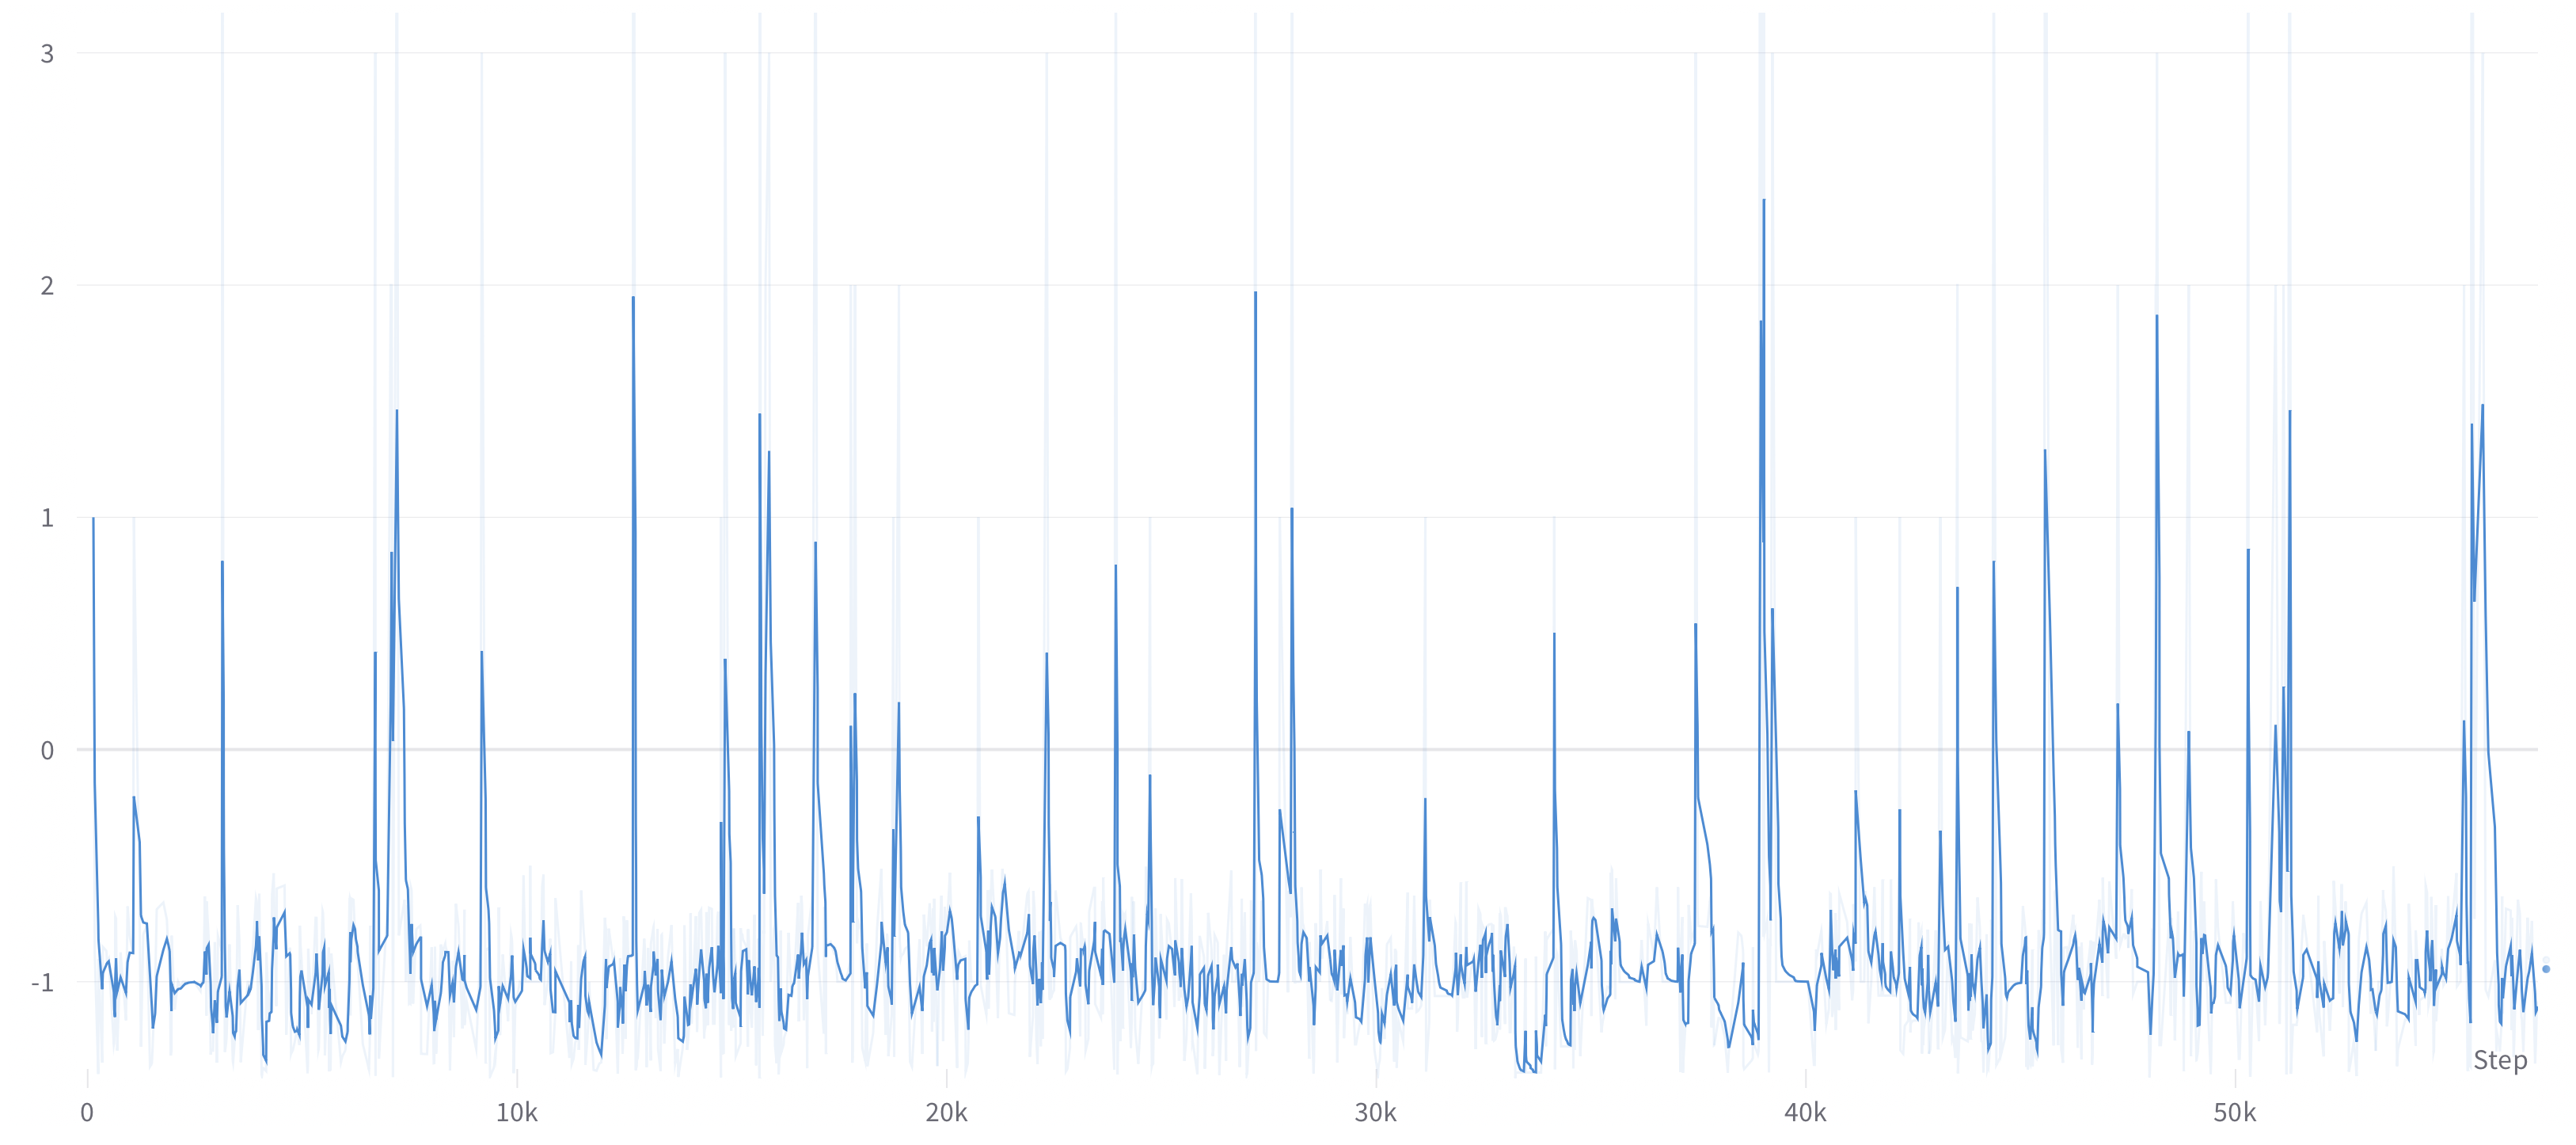
\includegraphics[width=\textwidth]{img/rewards_50_epochs.png}
			\caption{Total reward after 50 epochs}
			\label{fig:g}
		\end{subfigure}
		\hfill
		\begin{subfigure}[b]{0.45\textwidth}
			\centering
			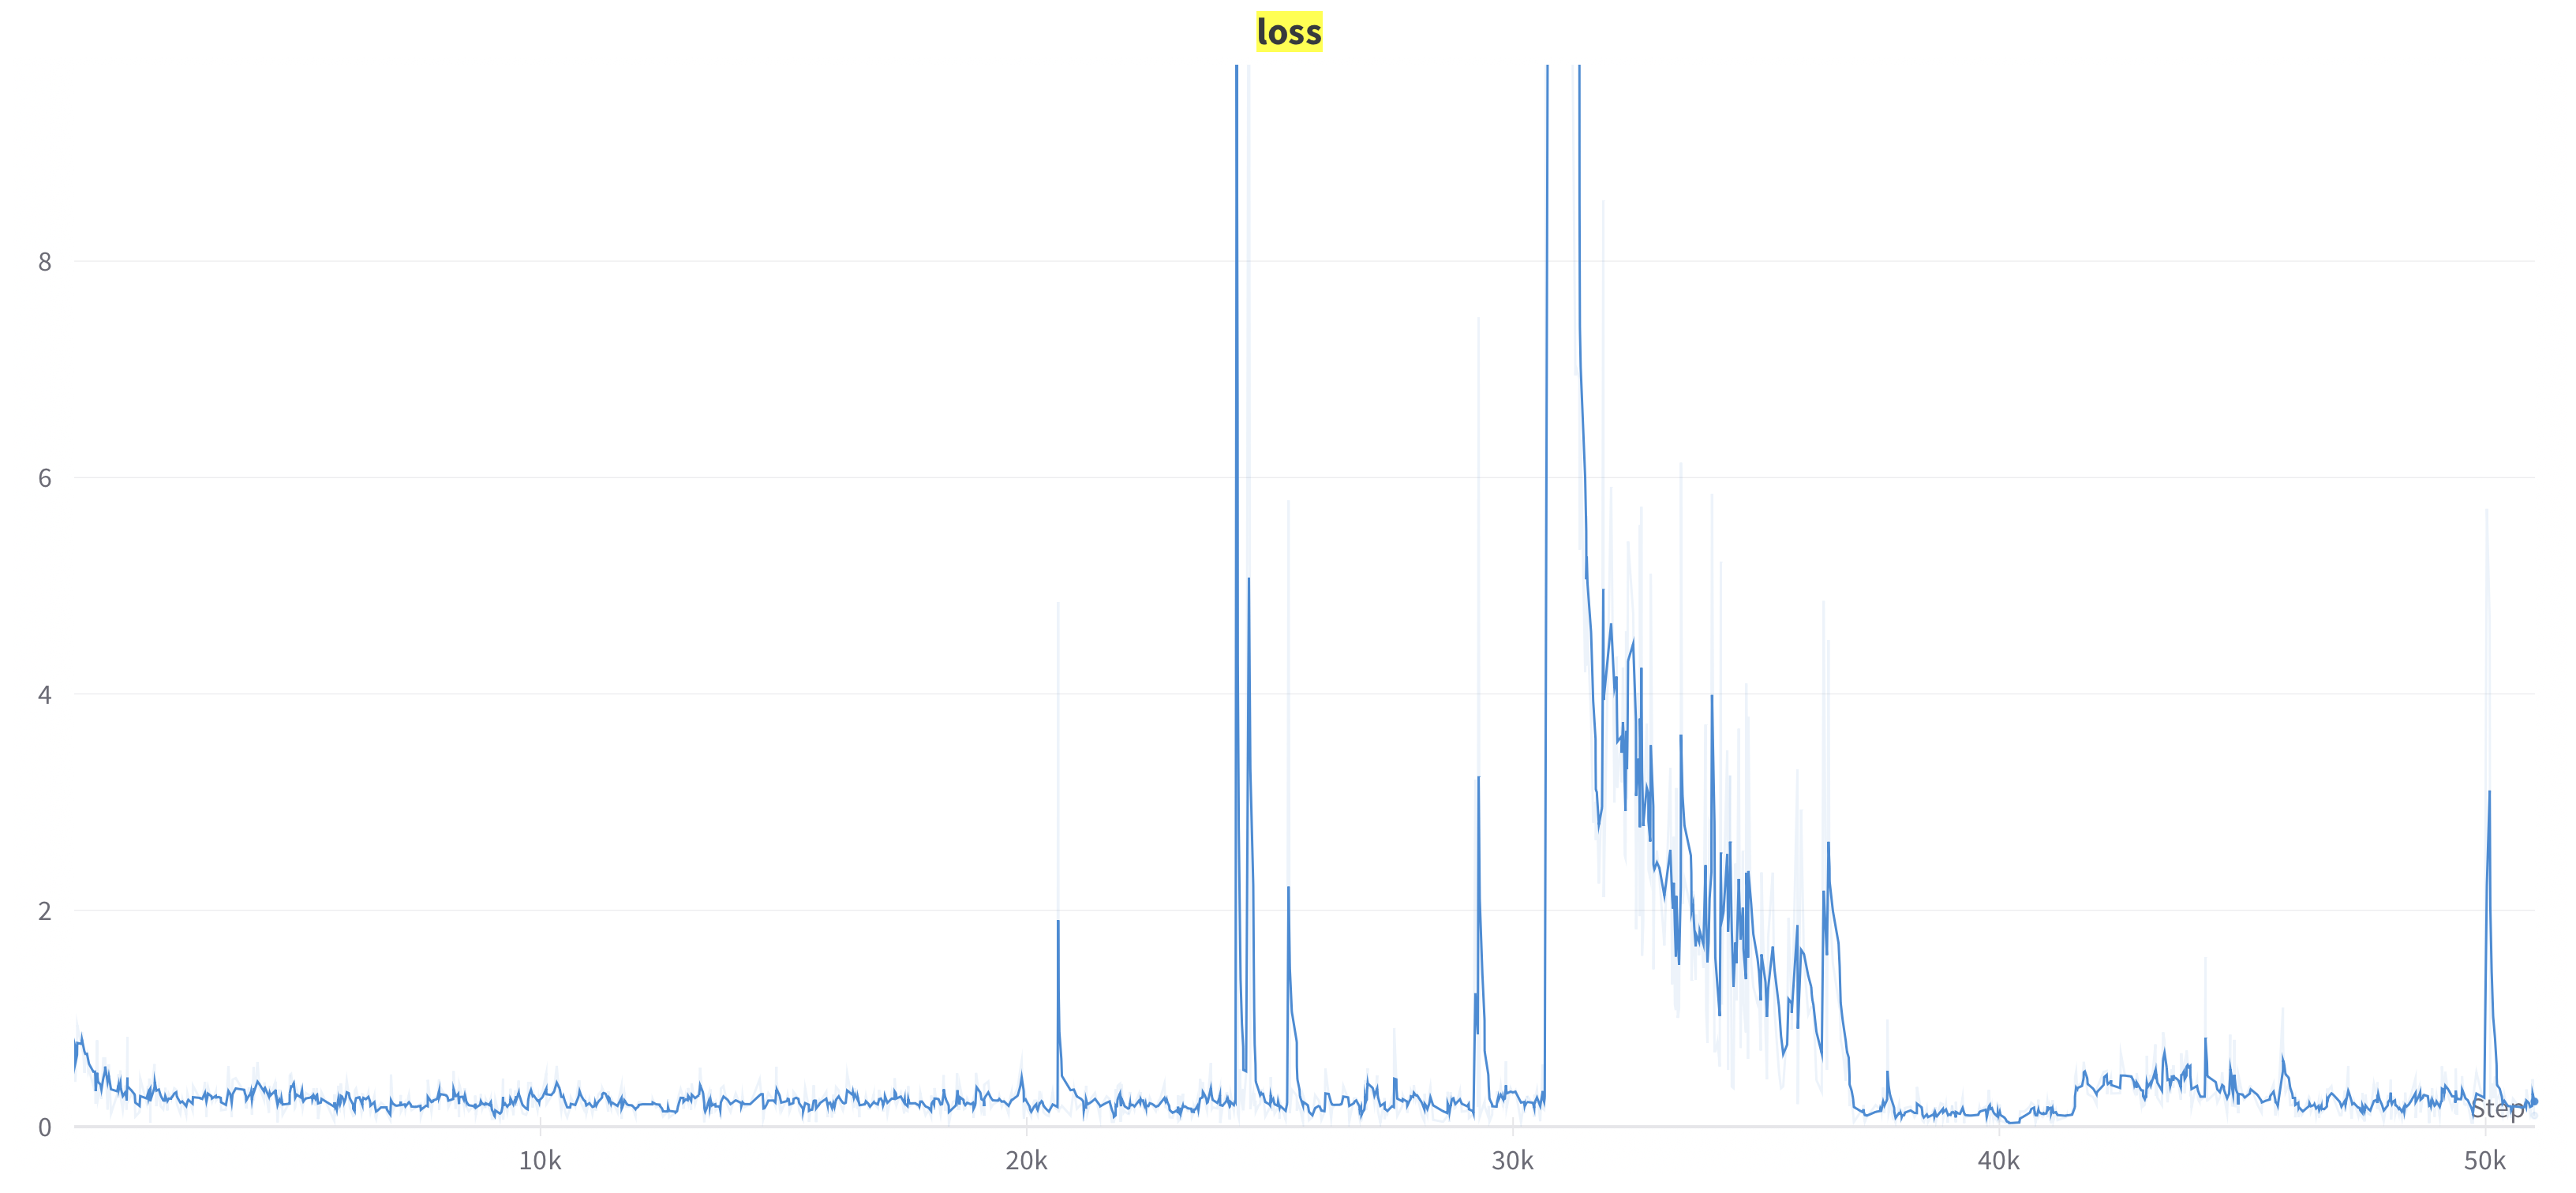
\includegraphics[width=\textwidth]{img/loss_50_epochs.png}
			\caption{Total loss after 50 epochs}
			\label{fig:h}
		\end{subfigure}
		\hfill
		\begin{subfigure}[b]{0.45\textwidth}
			\centering
			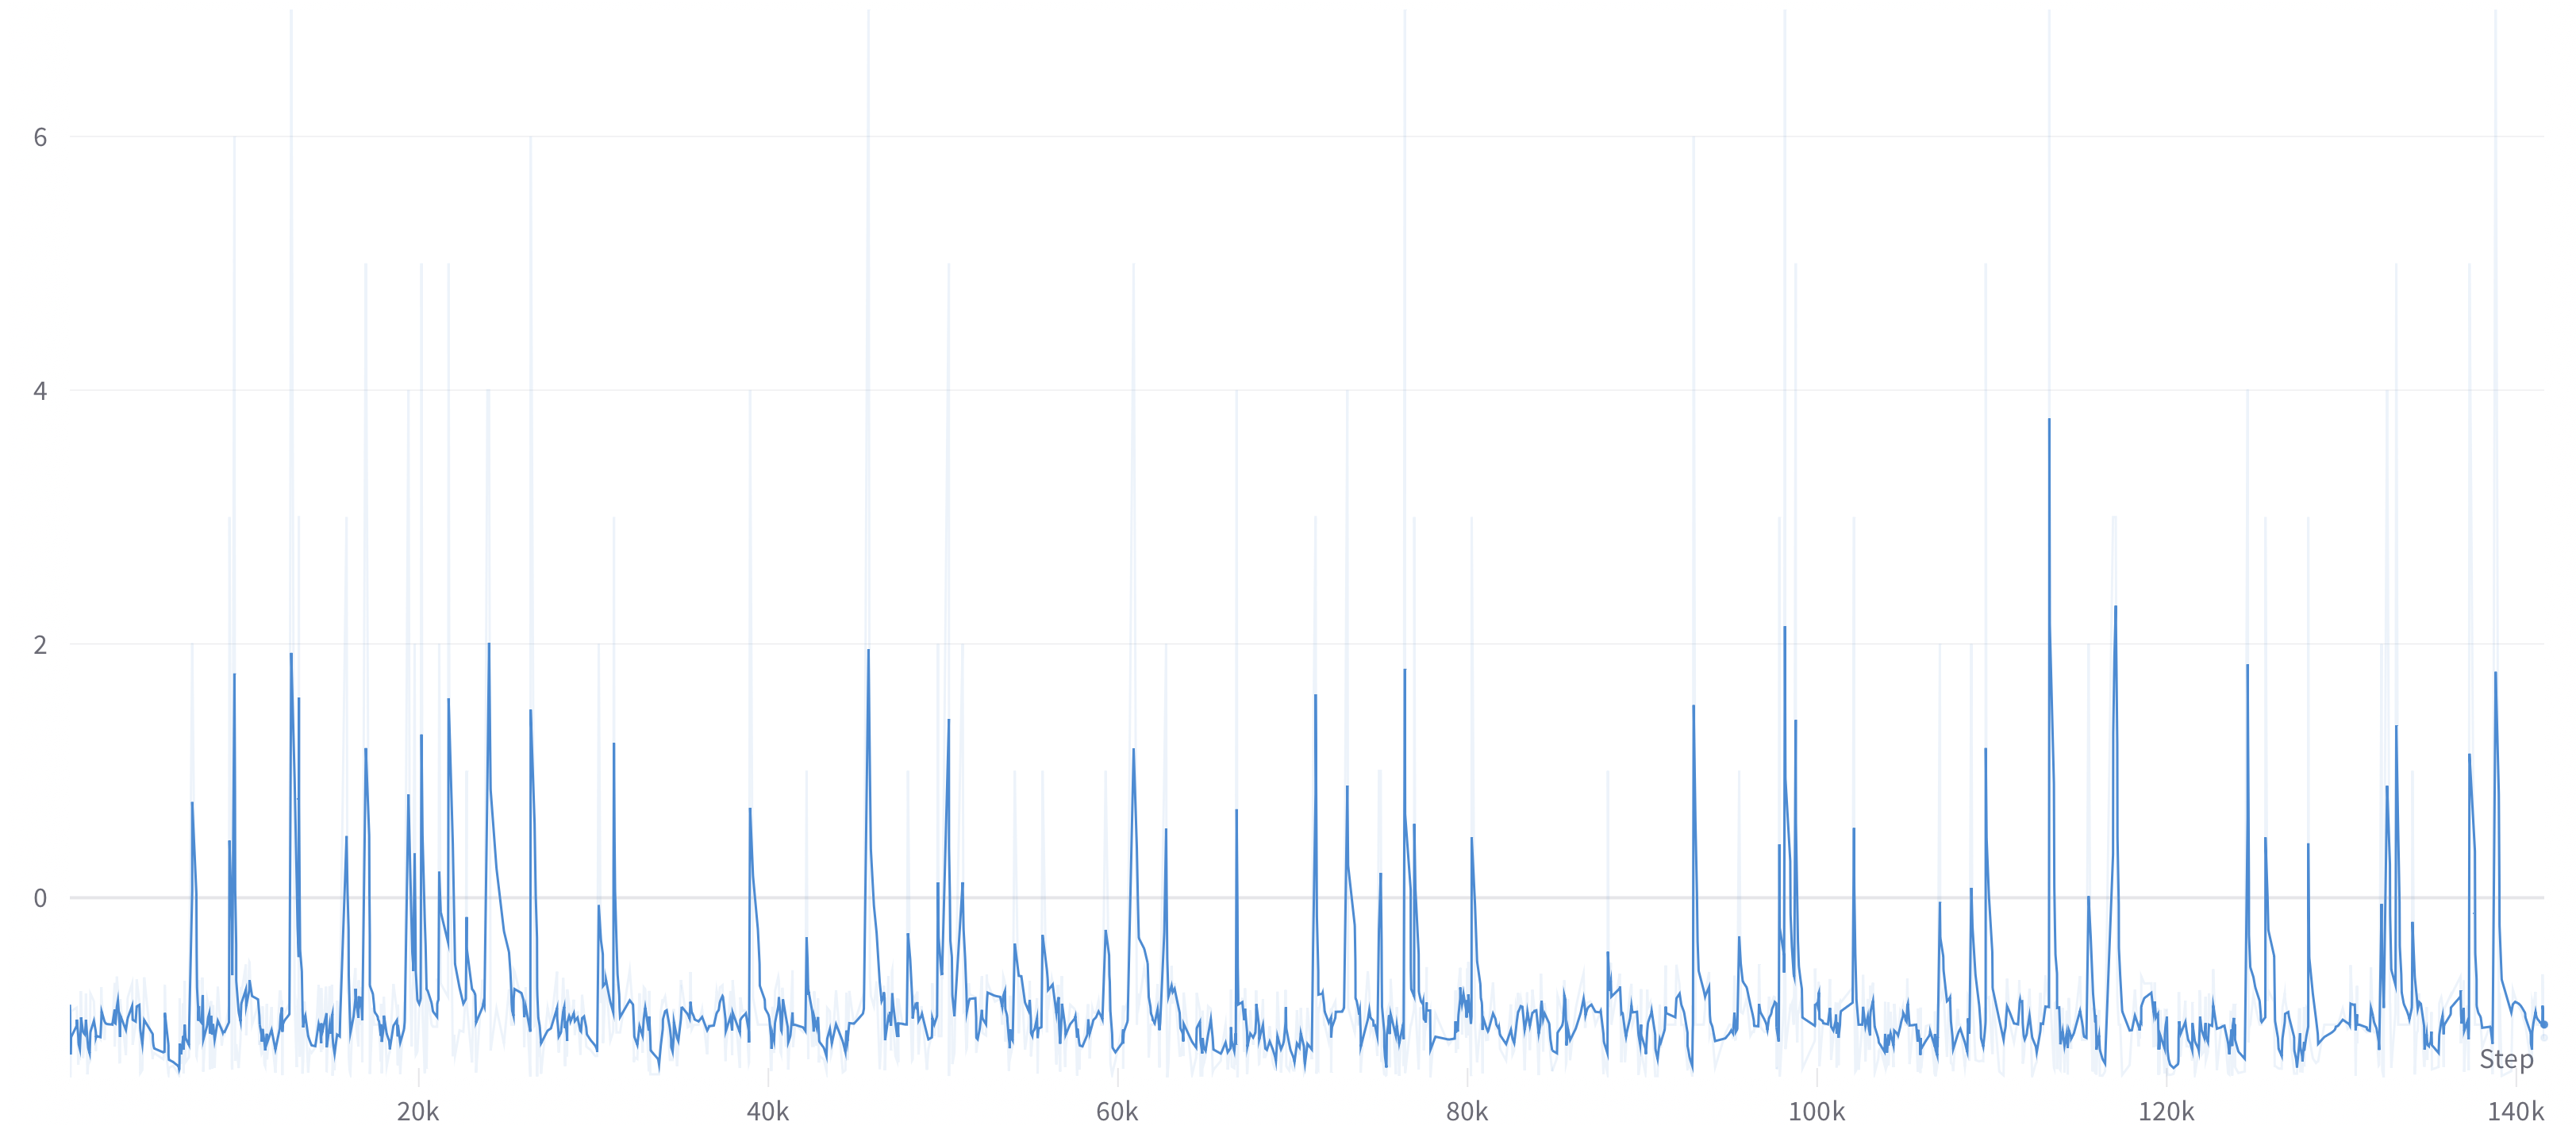
\includegraphics[width=\textwidth]{img/rewards.png}
			\caption{Total reward after 150 epochs} 
			\label{fig:i}
		\end{subfigure}
		\hfill
		\begin{subfigure}[b]{0.45\textwidth}
			\centering
			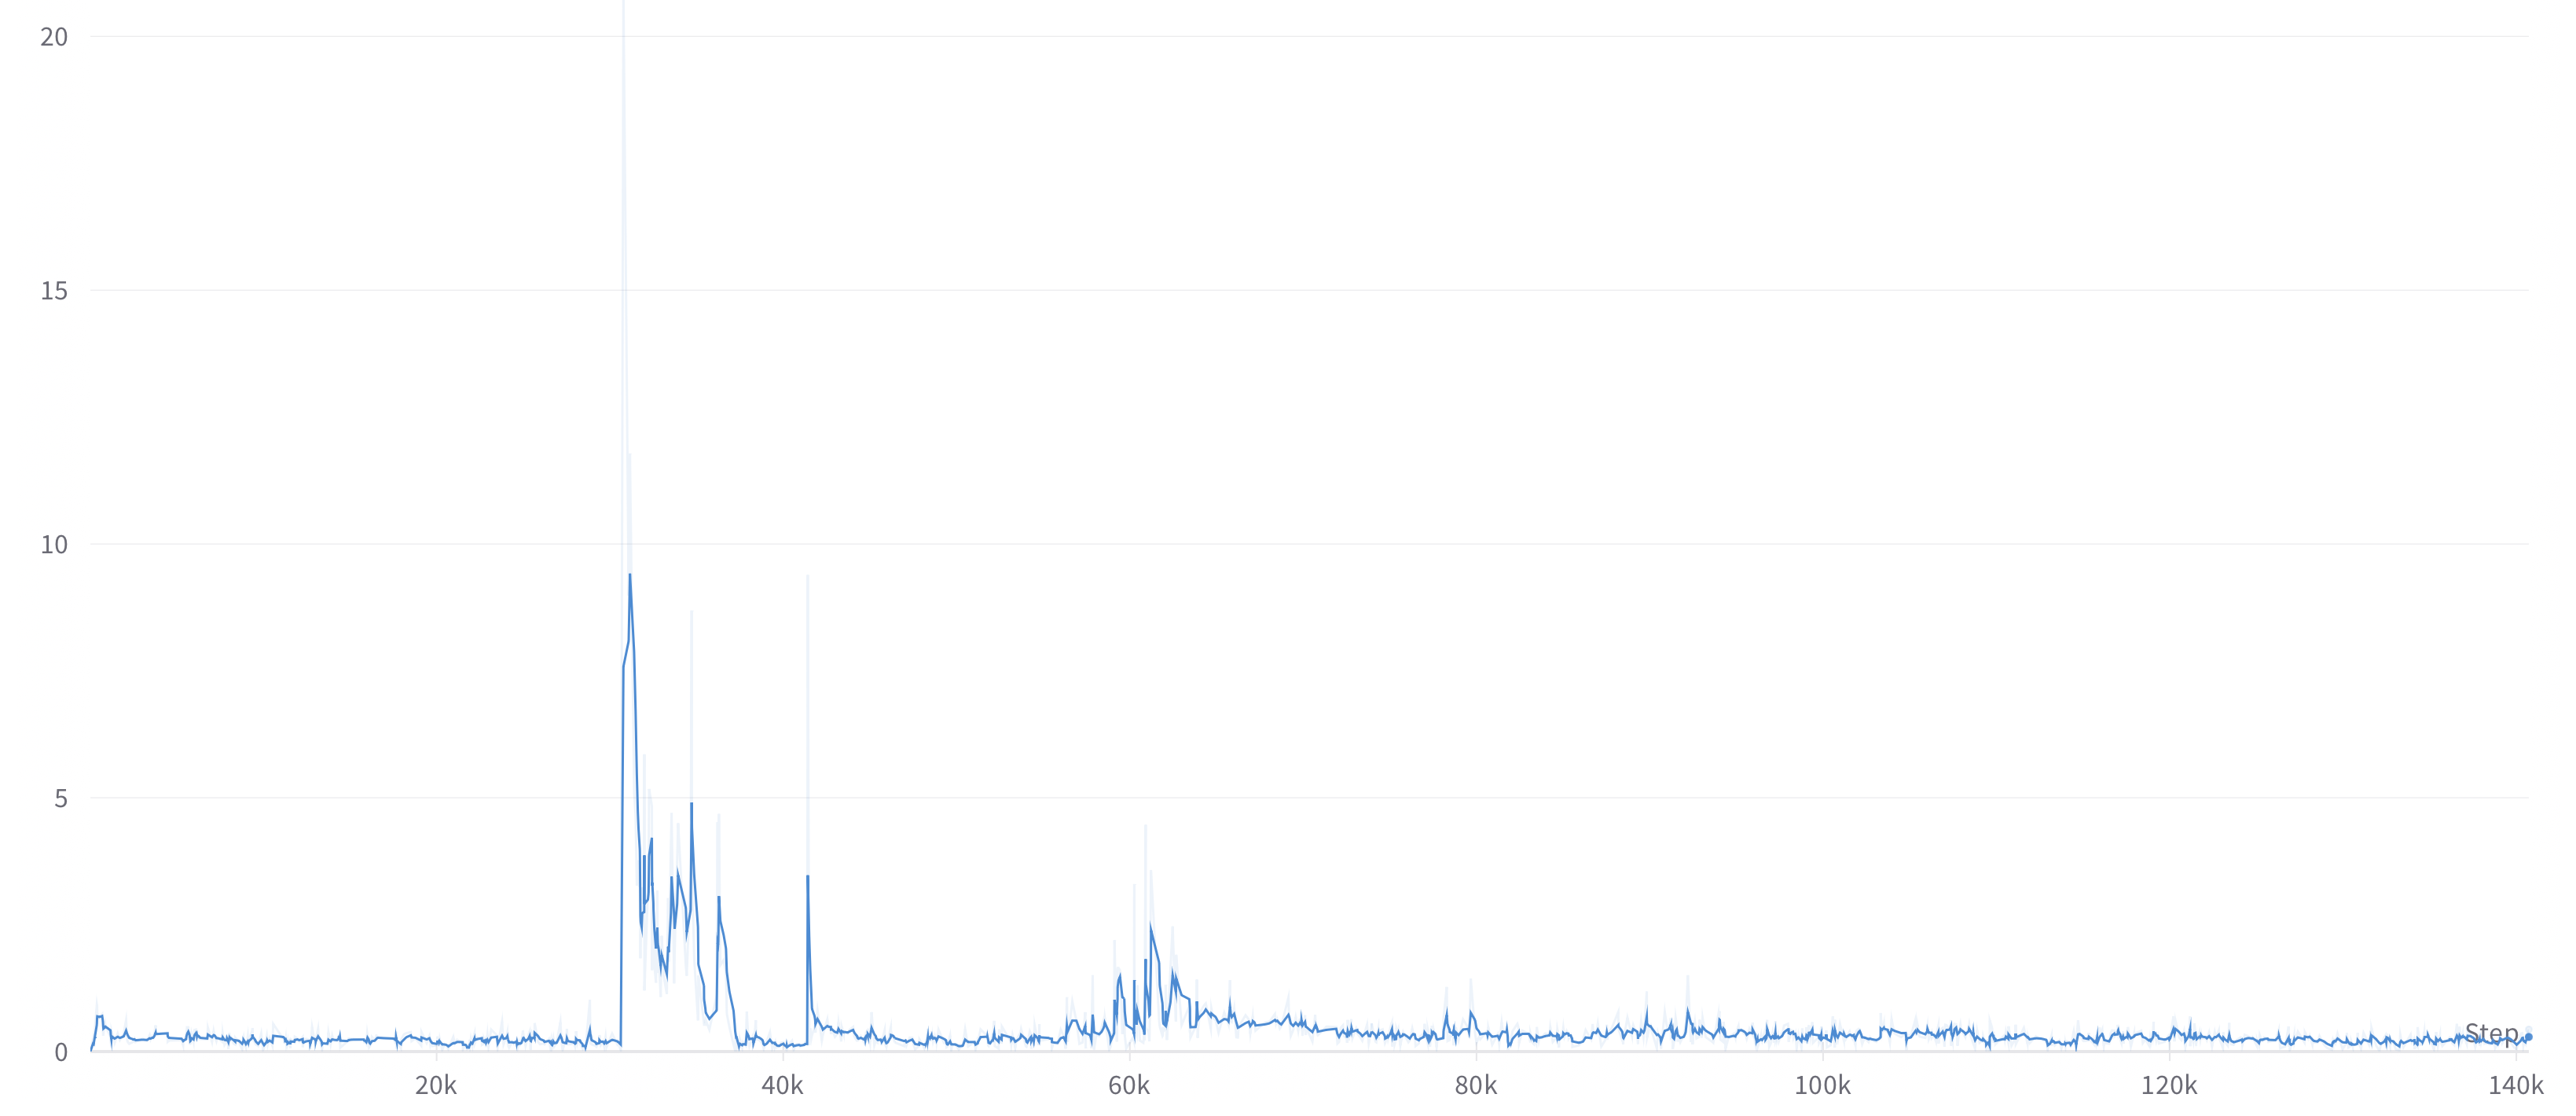
\includegraphics[width=\textwidth]{img/loss.png}
			\caption{Total loss after 150 epochs} 
			\label{fig:l}
		\end{subfigure}
		\caption{Reward and Loss comparison}
		\label{fig:s}
	\end{figure}

	\begin{figure}
		\centering
		\begin{subfigure}[b]{0.45\textwidth}
			\centering
			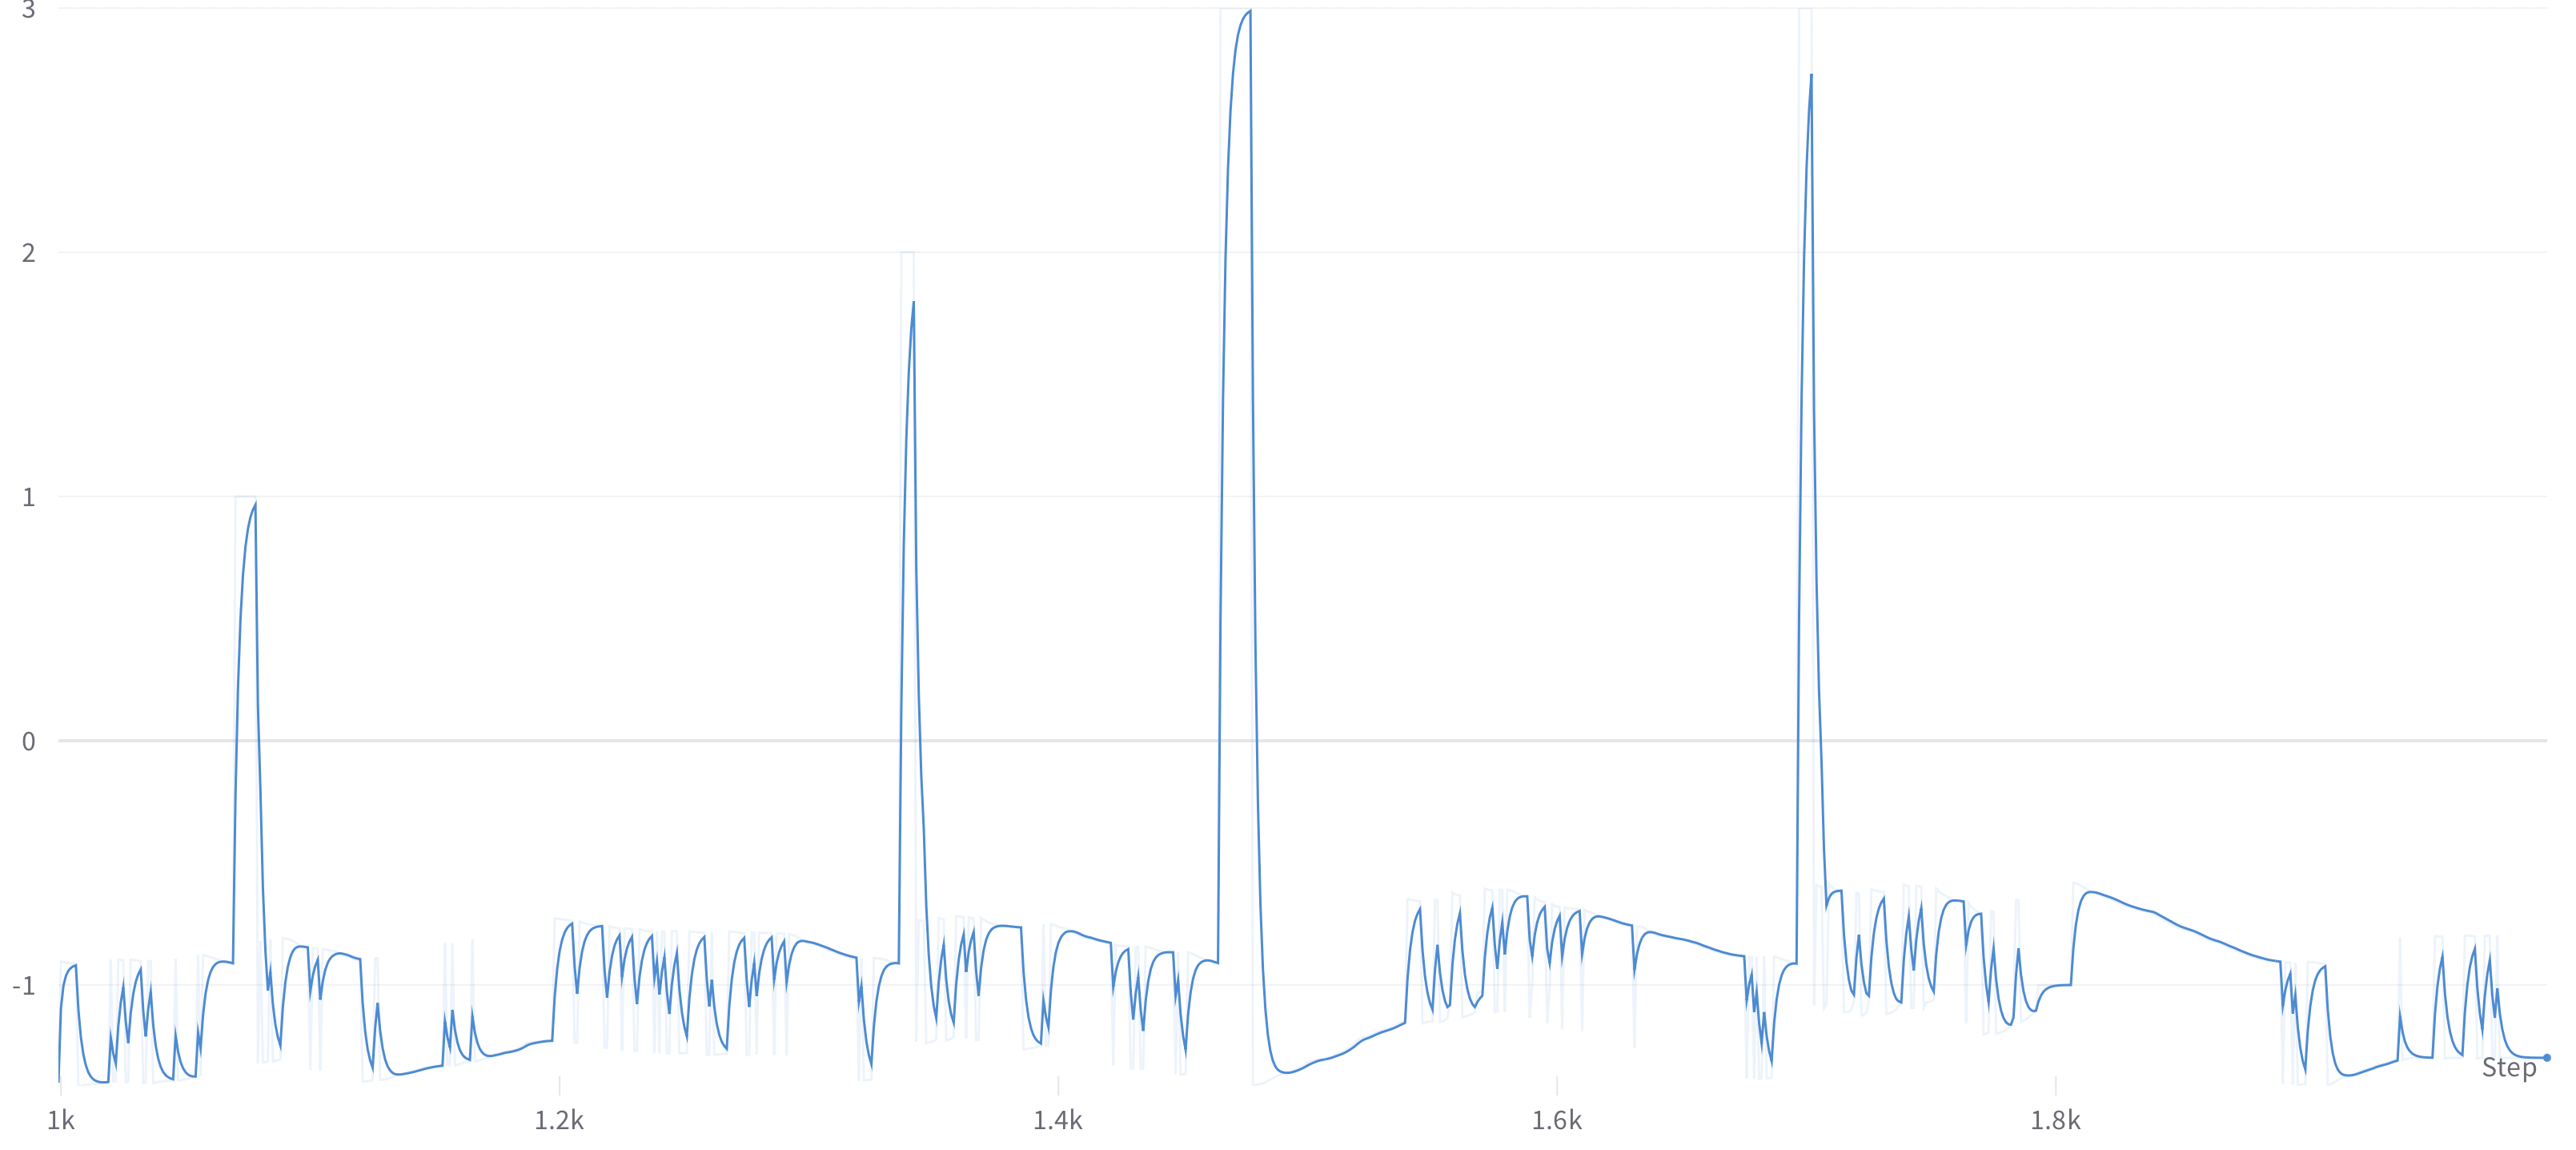
\includegraphics[width=\textwidth]{img/mean_reward_1_epoch.png}
			\caption{Mean Reward Epoch 1}
			\label{fig:d}
		\end{subfigure}
		\hfill
		\begin{subfigure}[b]{0.45\textwidth}
			\centering
			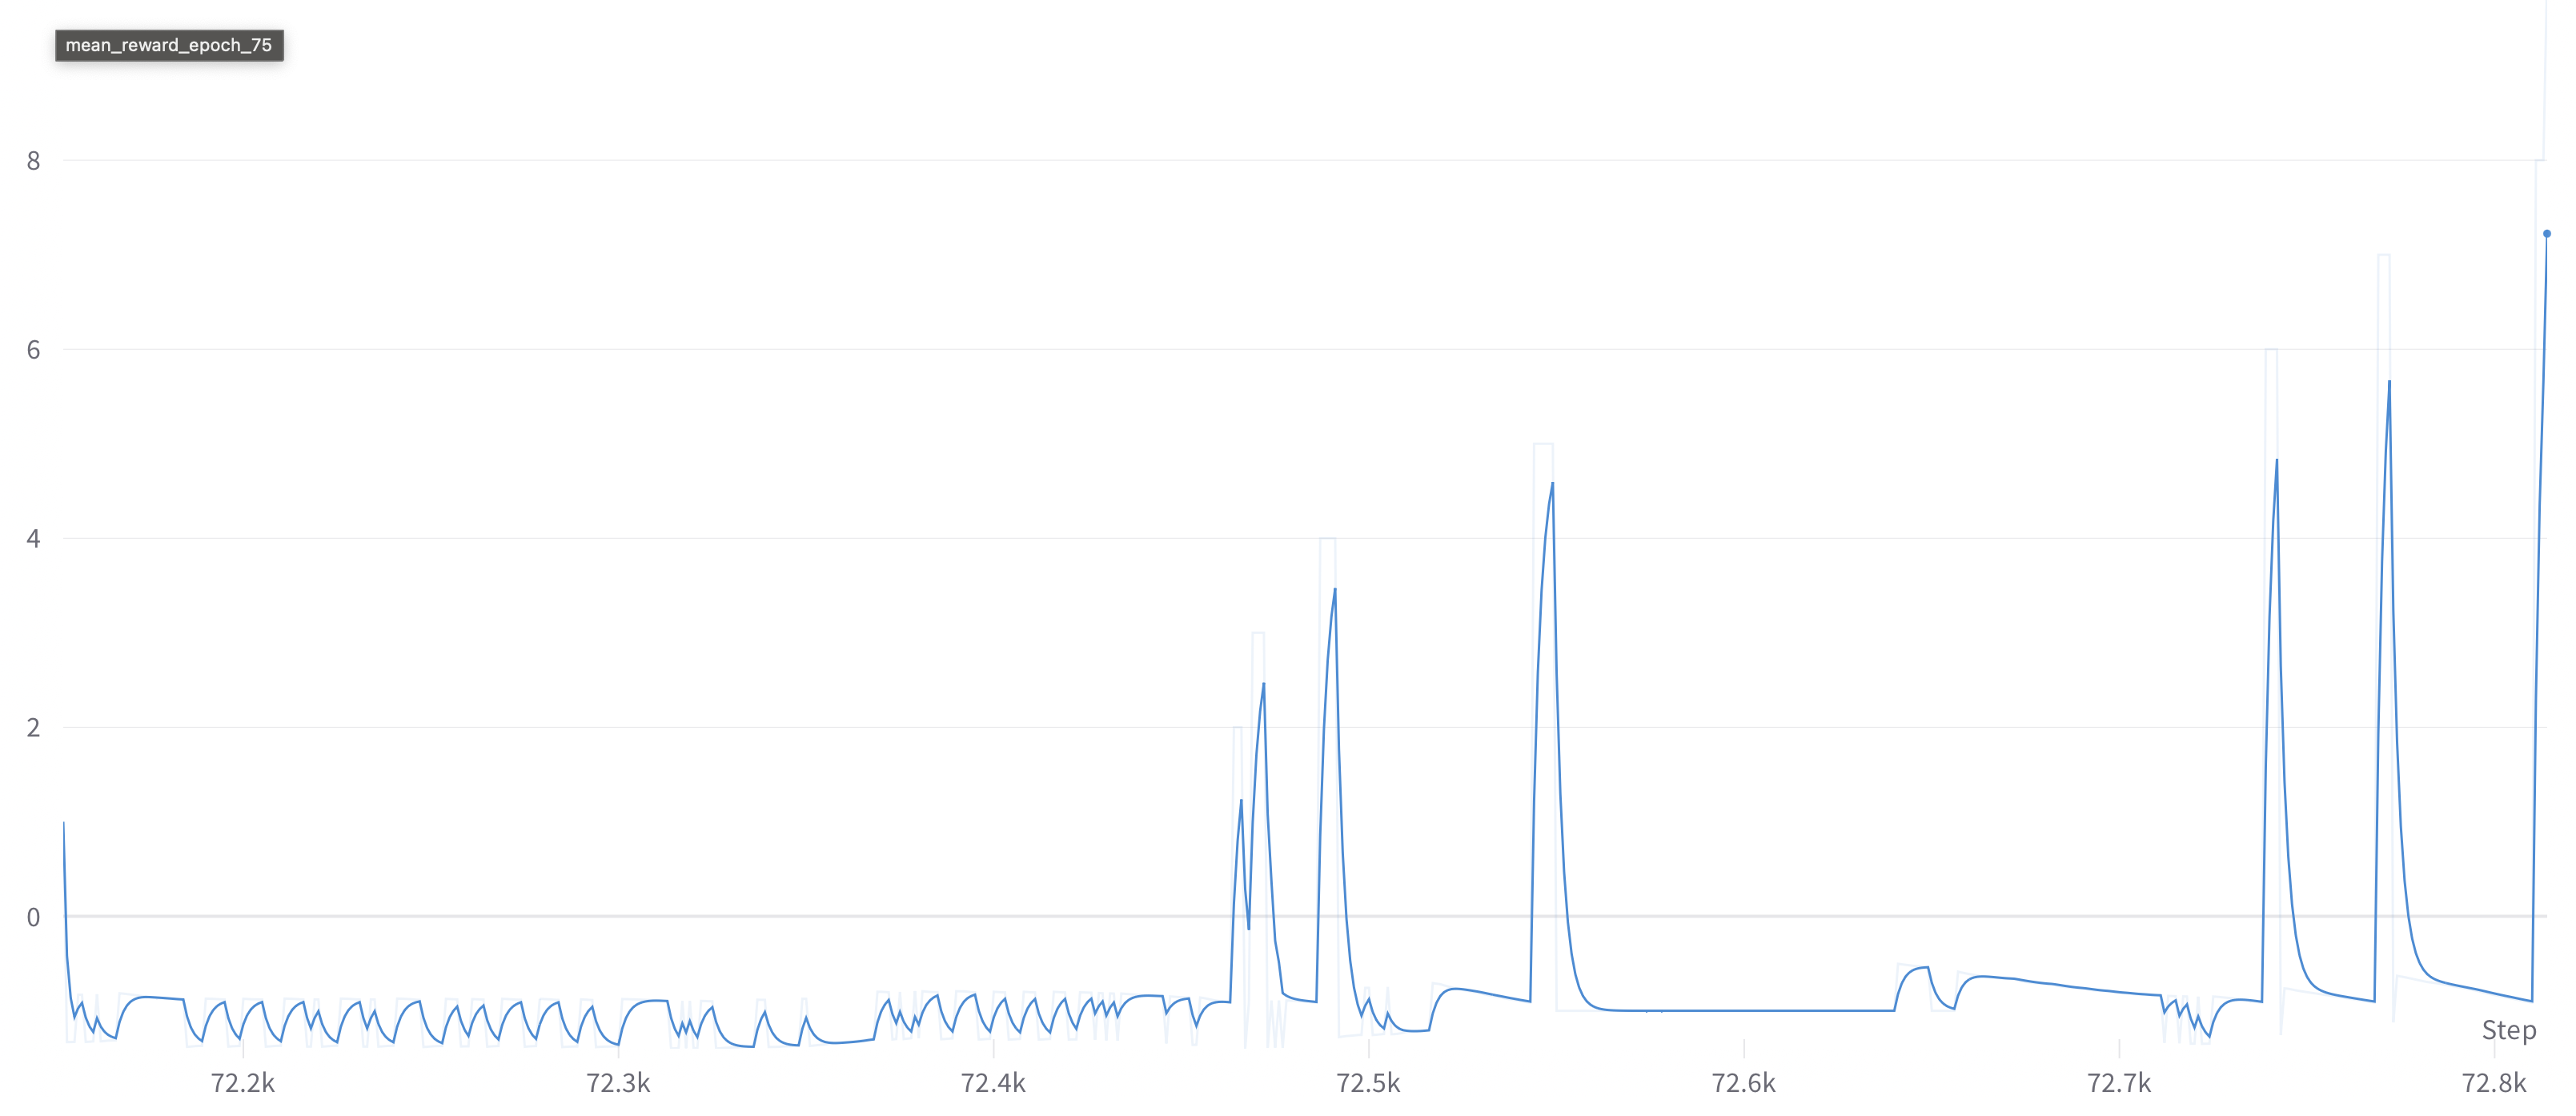
\includegraphics[width=\textwidth]{img/mean_reward_70_epoch.png}
			\caption{Mean Reward Epoch 70}
			\label{fig:e}
		\end{subfigure}
		\hfill
		\begin{subfigure}[b]{0.45\textwidth}
			\centering
			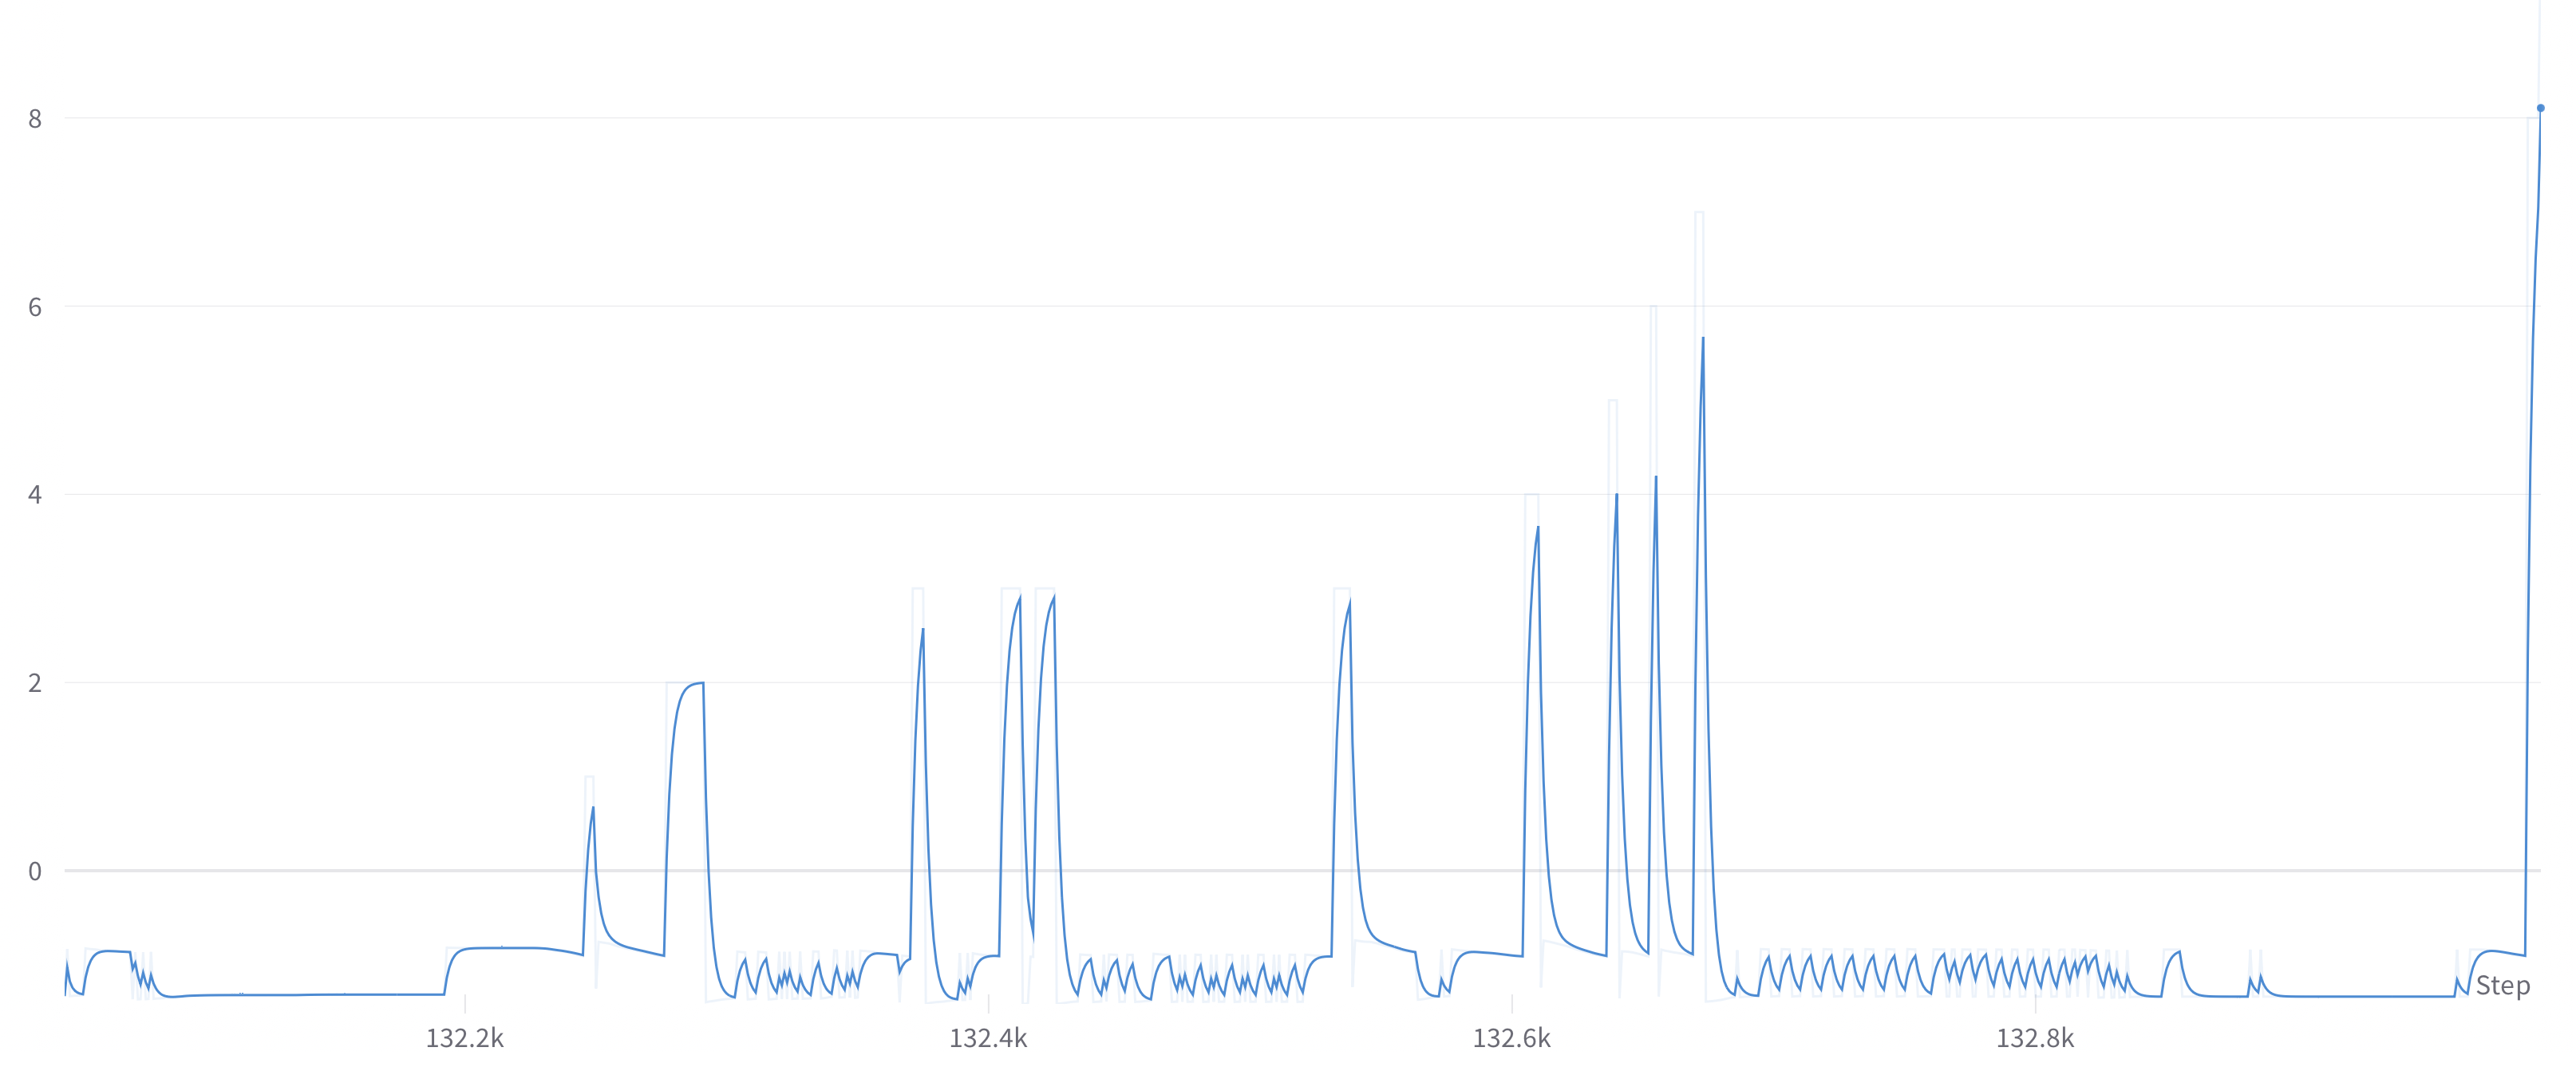
\includegraphics[width=\textwidth]{img/mean_reward_145_epoch.png}
			\caption{Mean Reward Epoch 145} 
			\label{fig:f}
		\end{subfigure}
		\caption{Mean rewards}
	\end{figure}

	\begin{figure}
		\centering
		\begin{subfigure}[b]{0.45\textwidth}
			\centering
			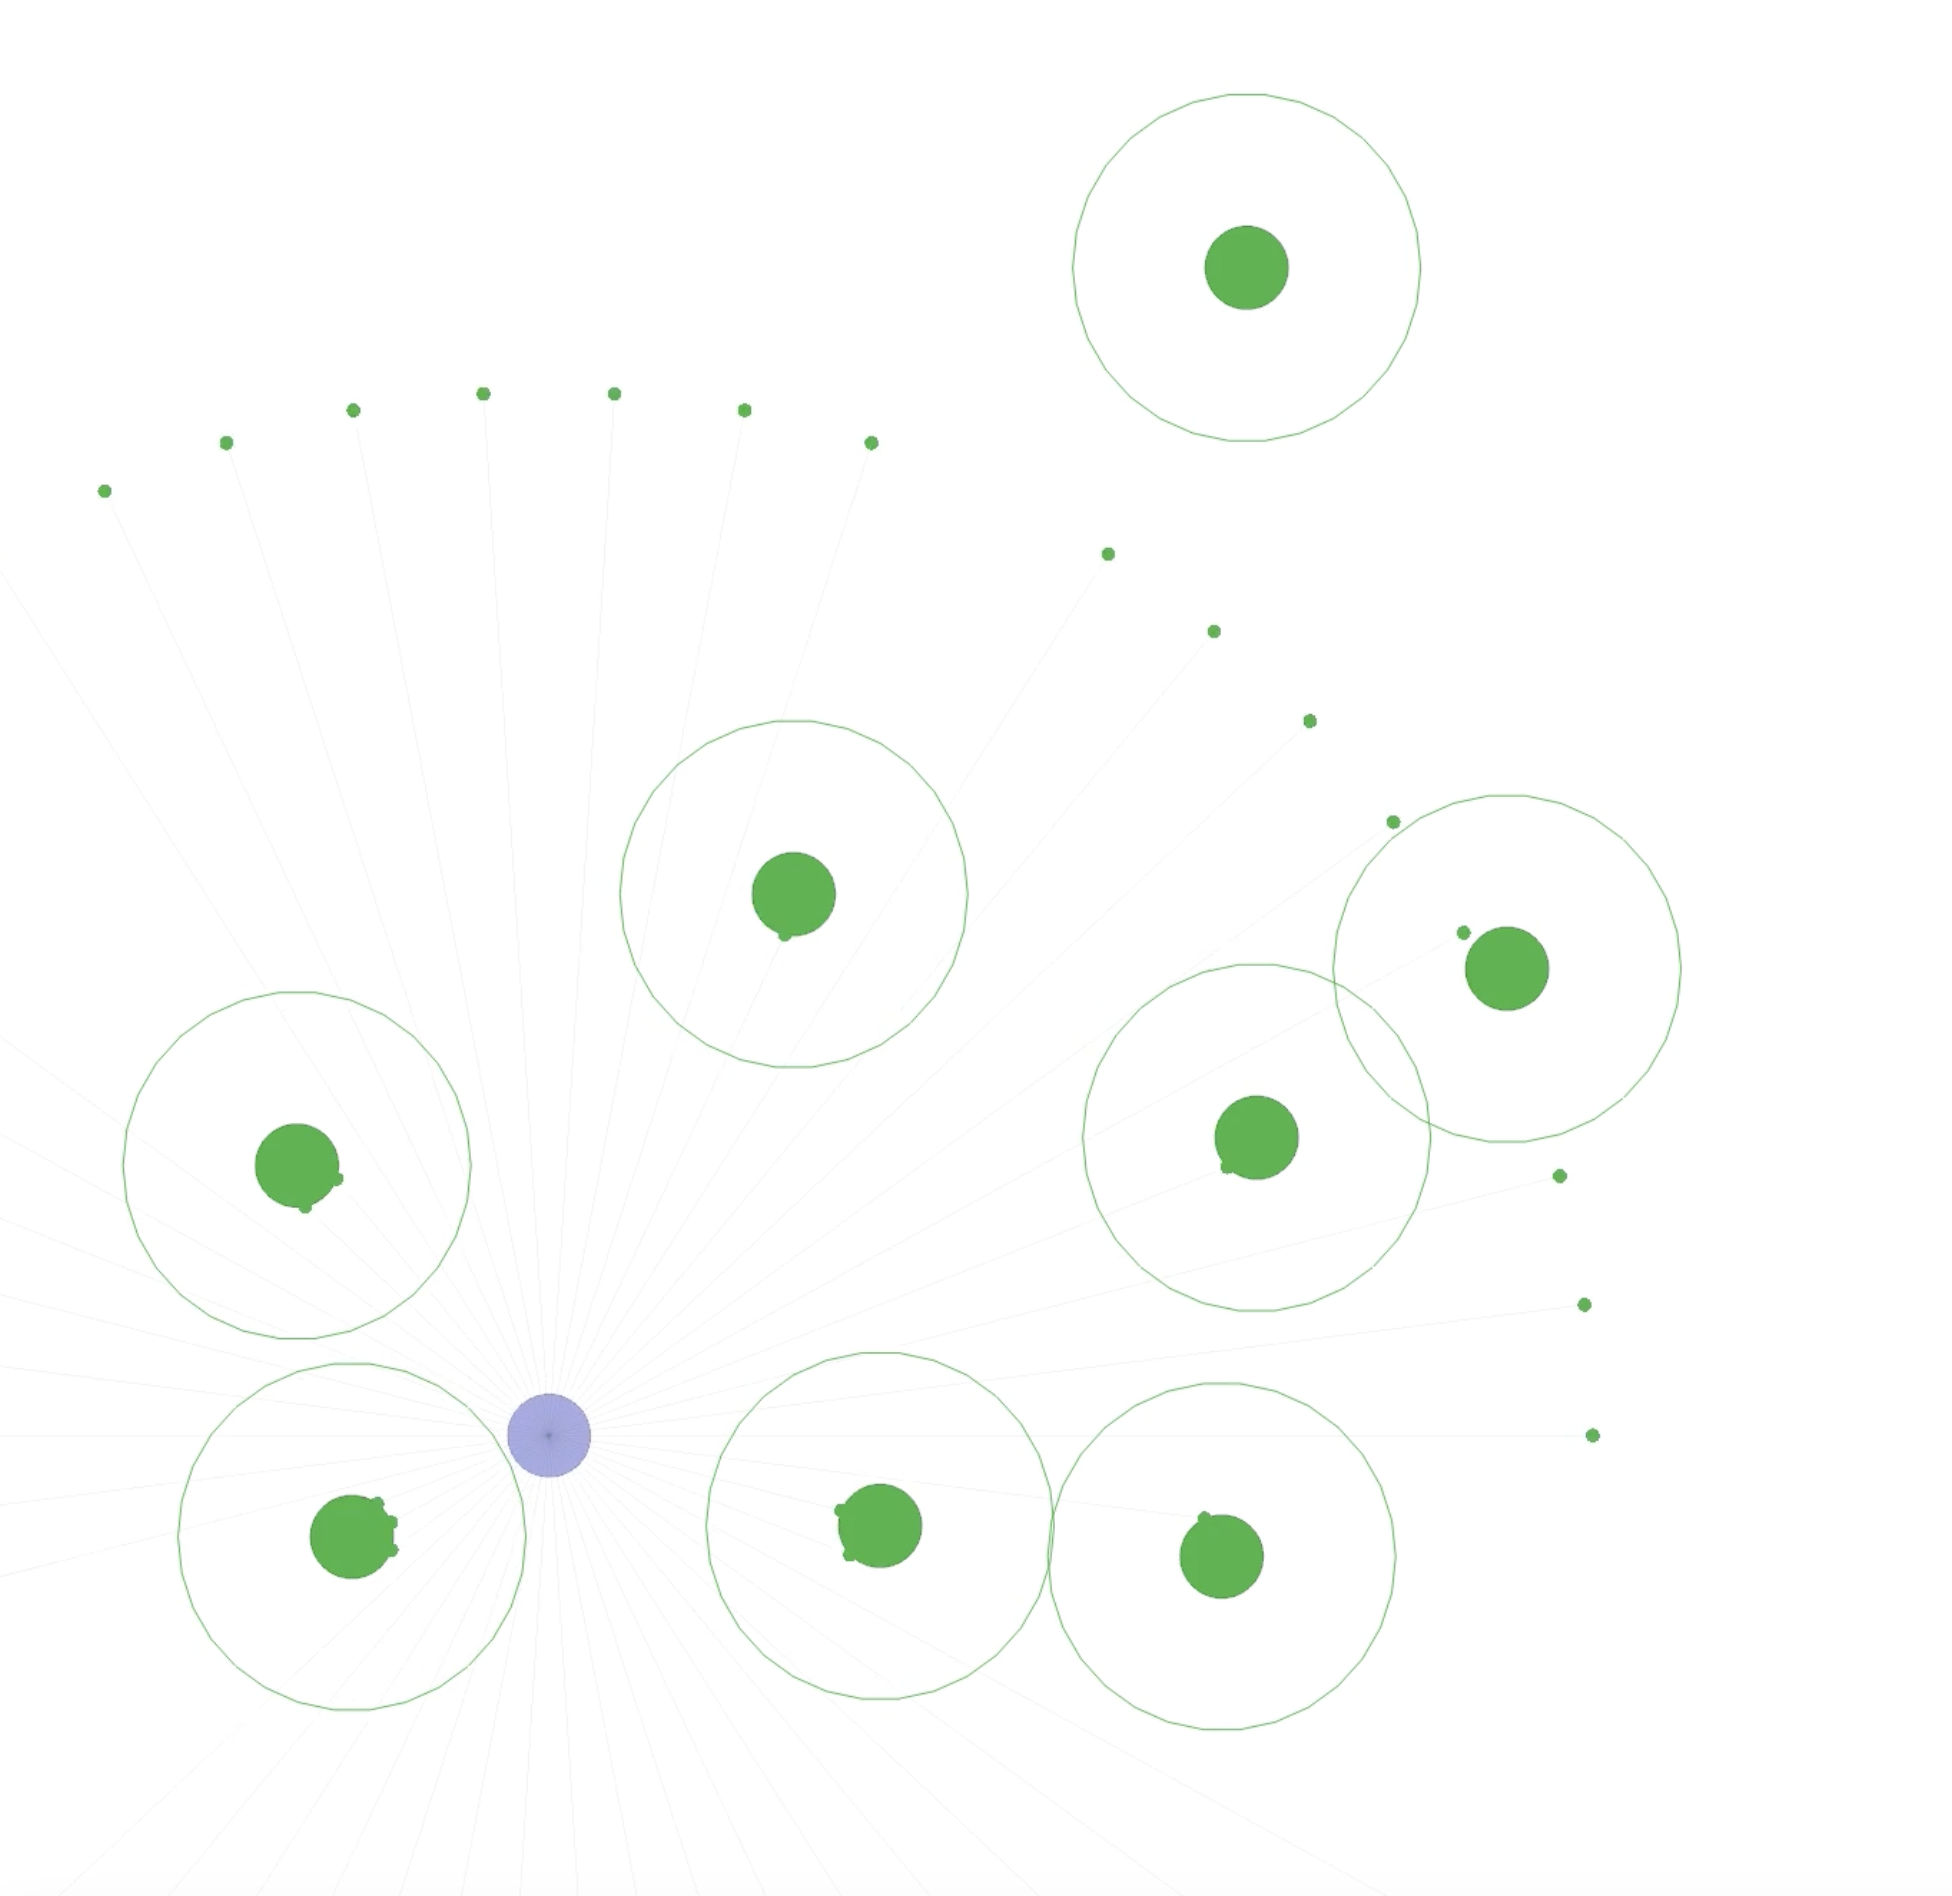
\includegraphics[width=\textwidth]{img/1_agent_1.png}
			\caption{Beginning of simulation}
		\end{subfigure}
		\hfill
		\begin{subfigure}[b]{0.45\textwidth}
			\centering
			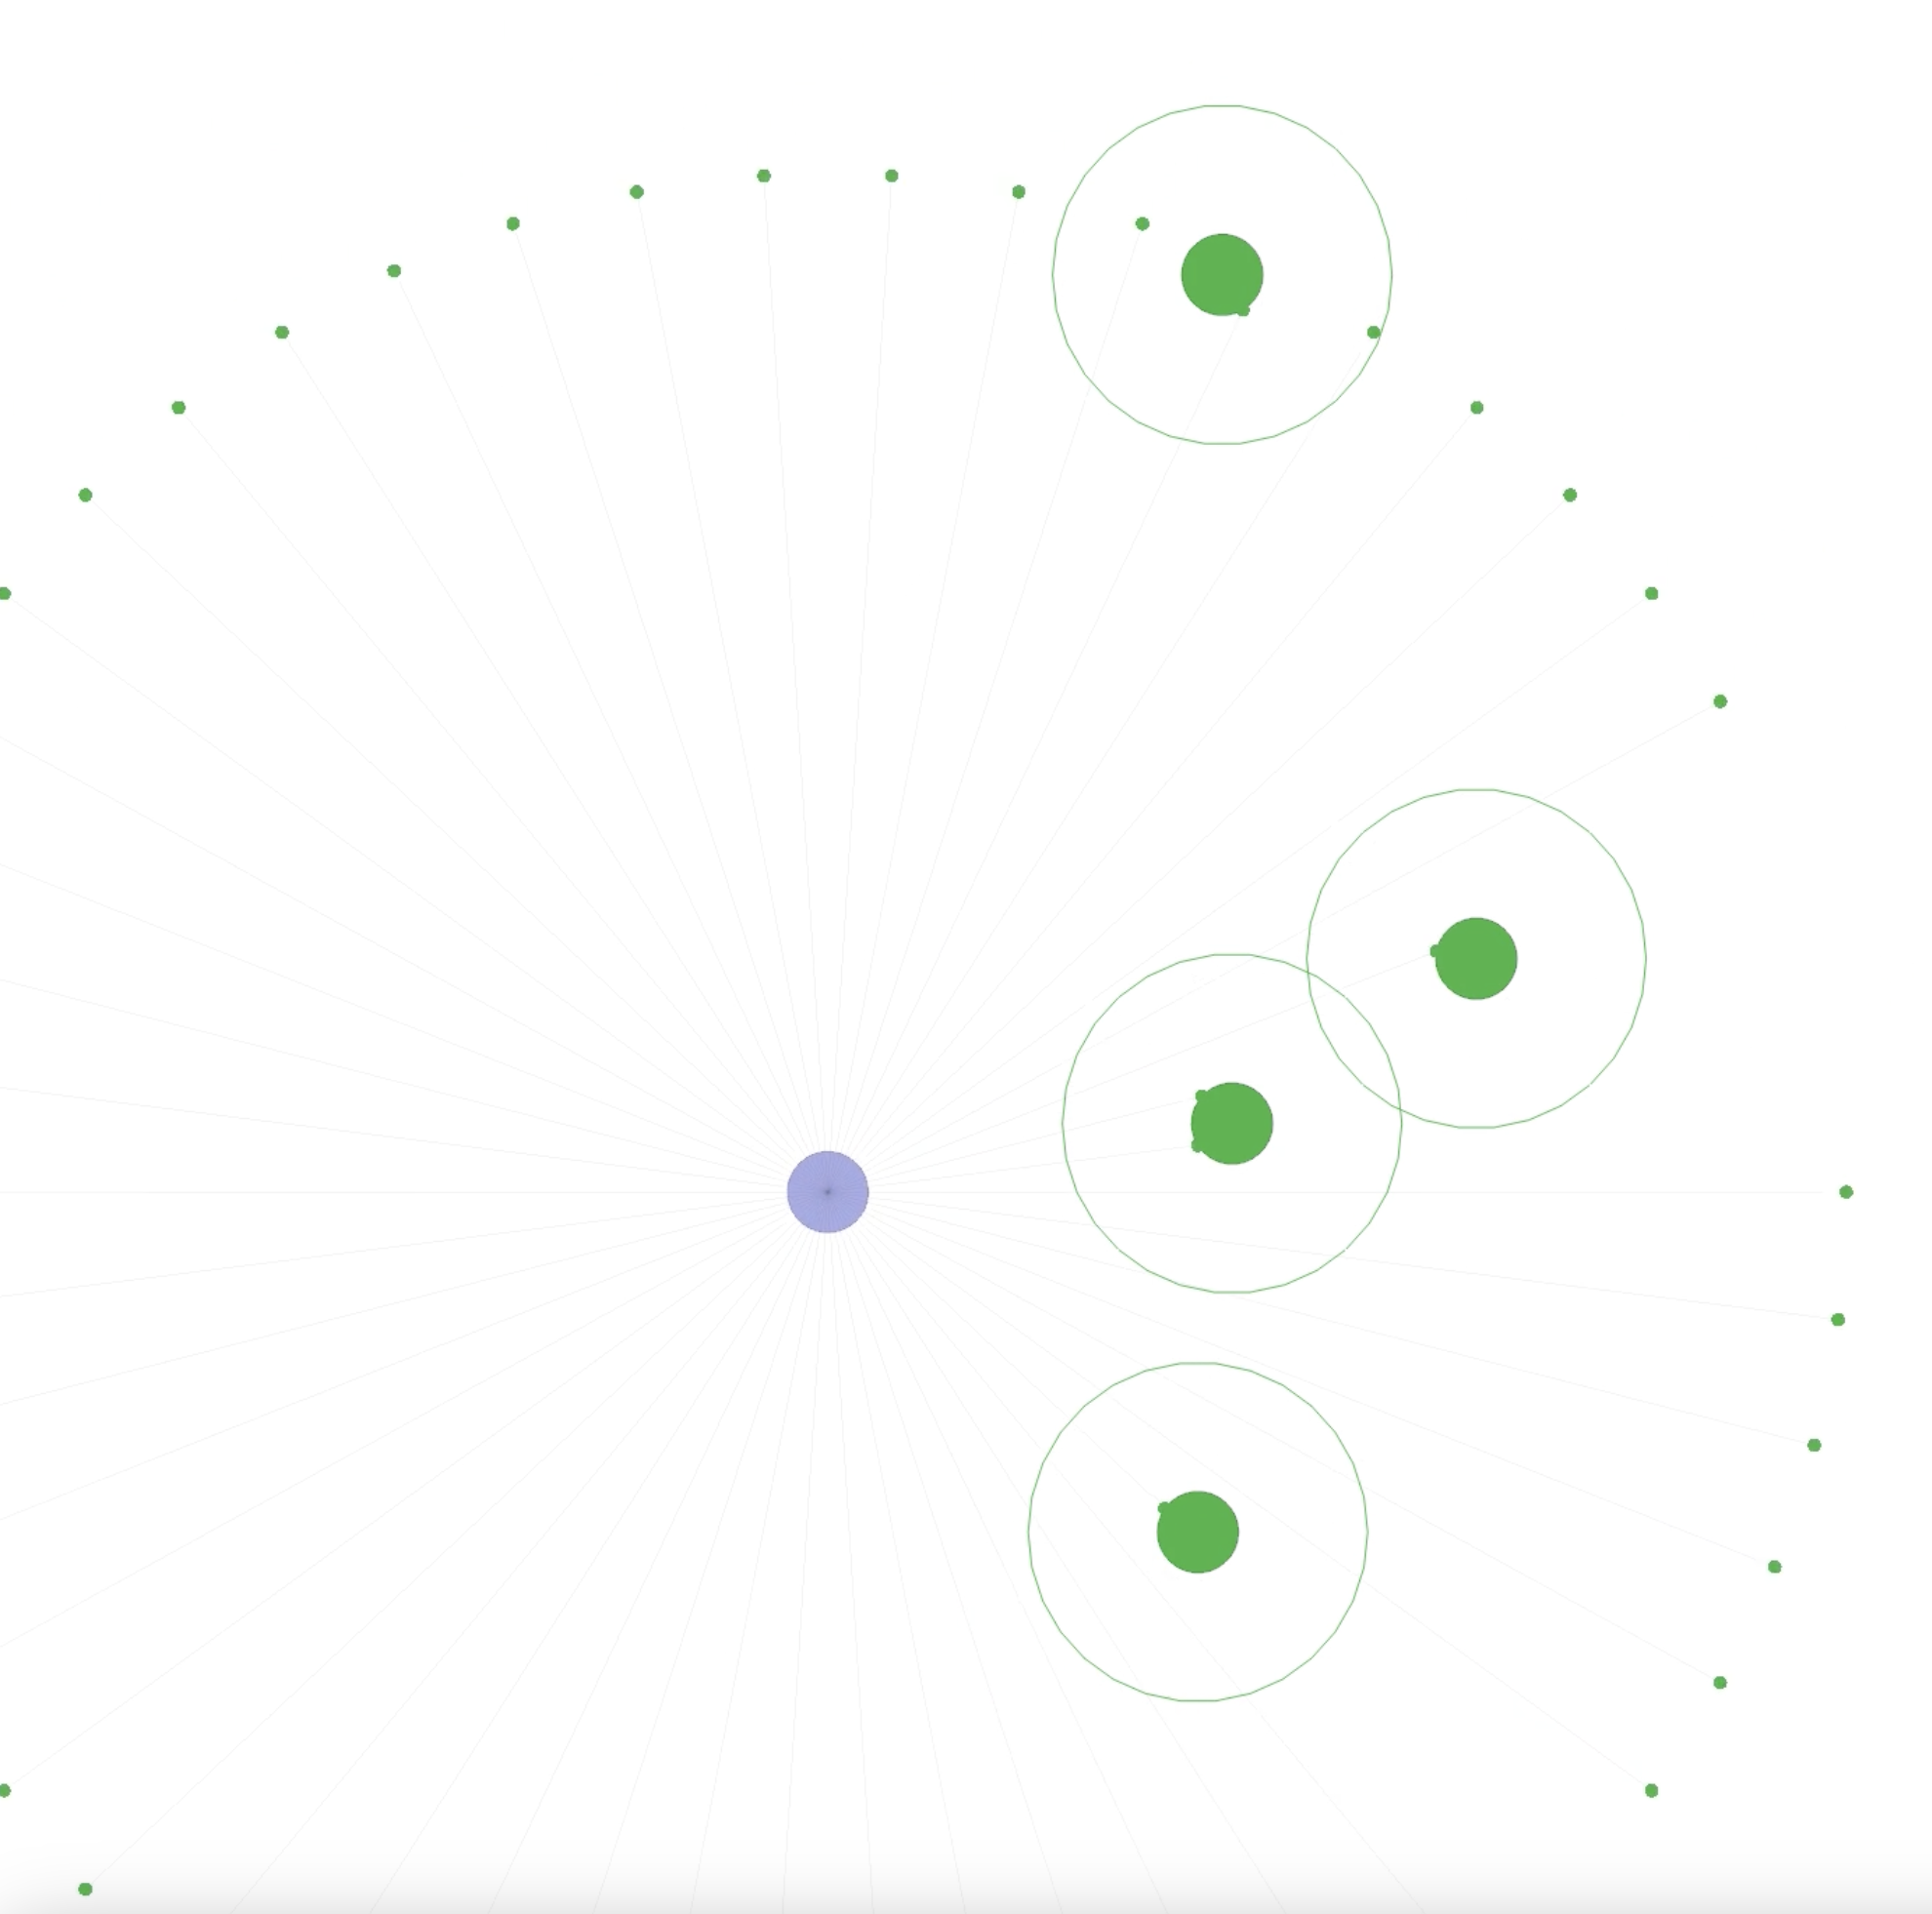
\includegraphics[width=\textwidth]{img/1_agent_2.png}
			\caption{Half simulation}
		\end{subfigure}
		\hfill
		\begin{subfigure}[b]{0.45\textwidth}
			\centering
			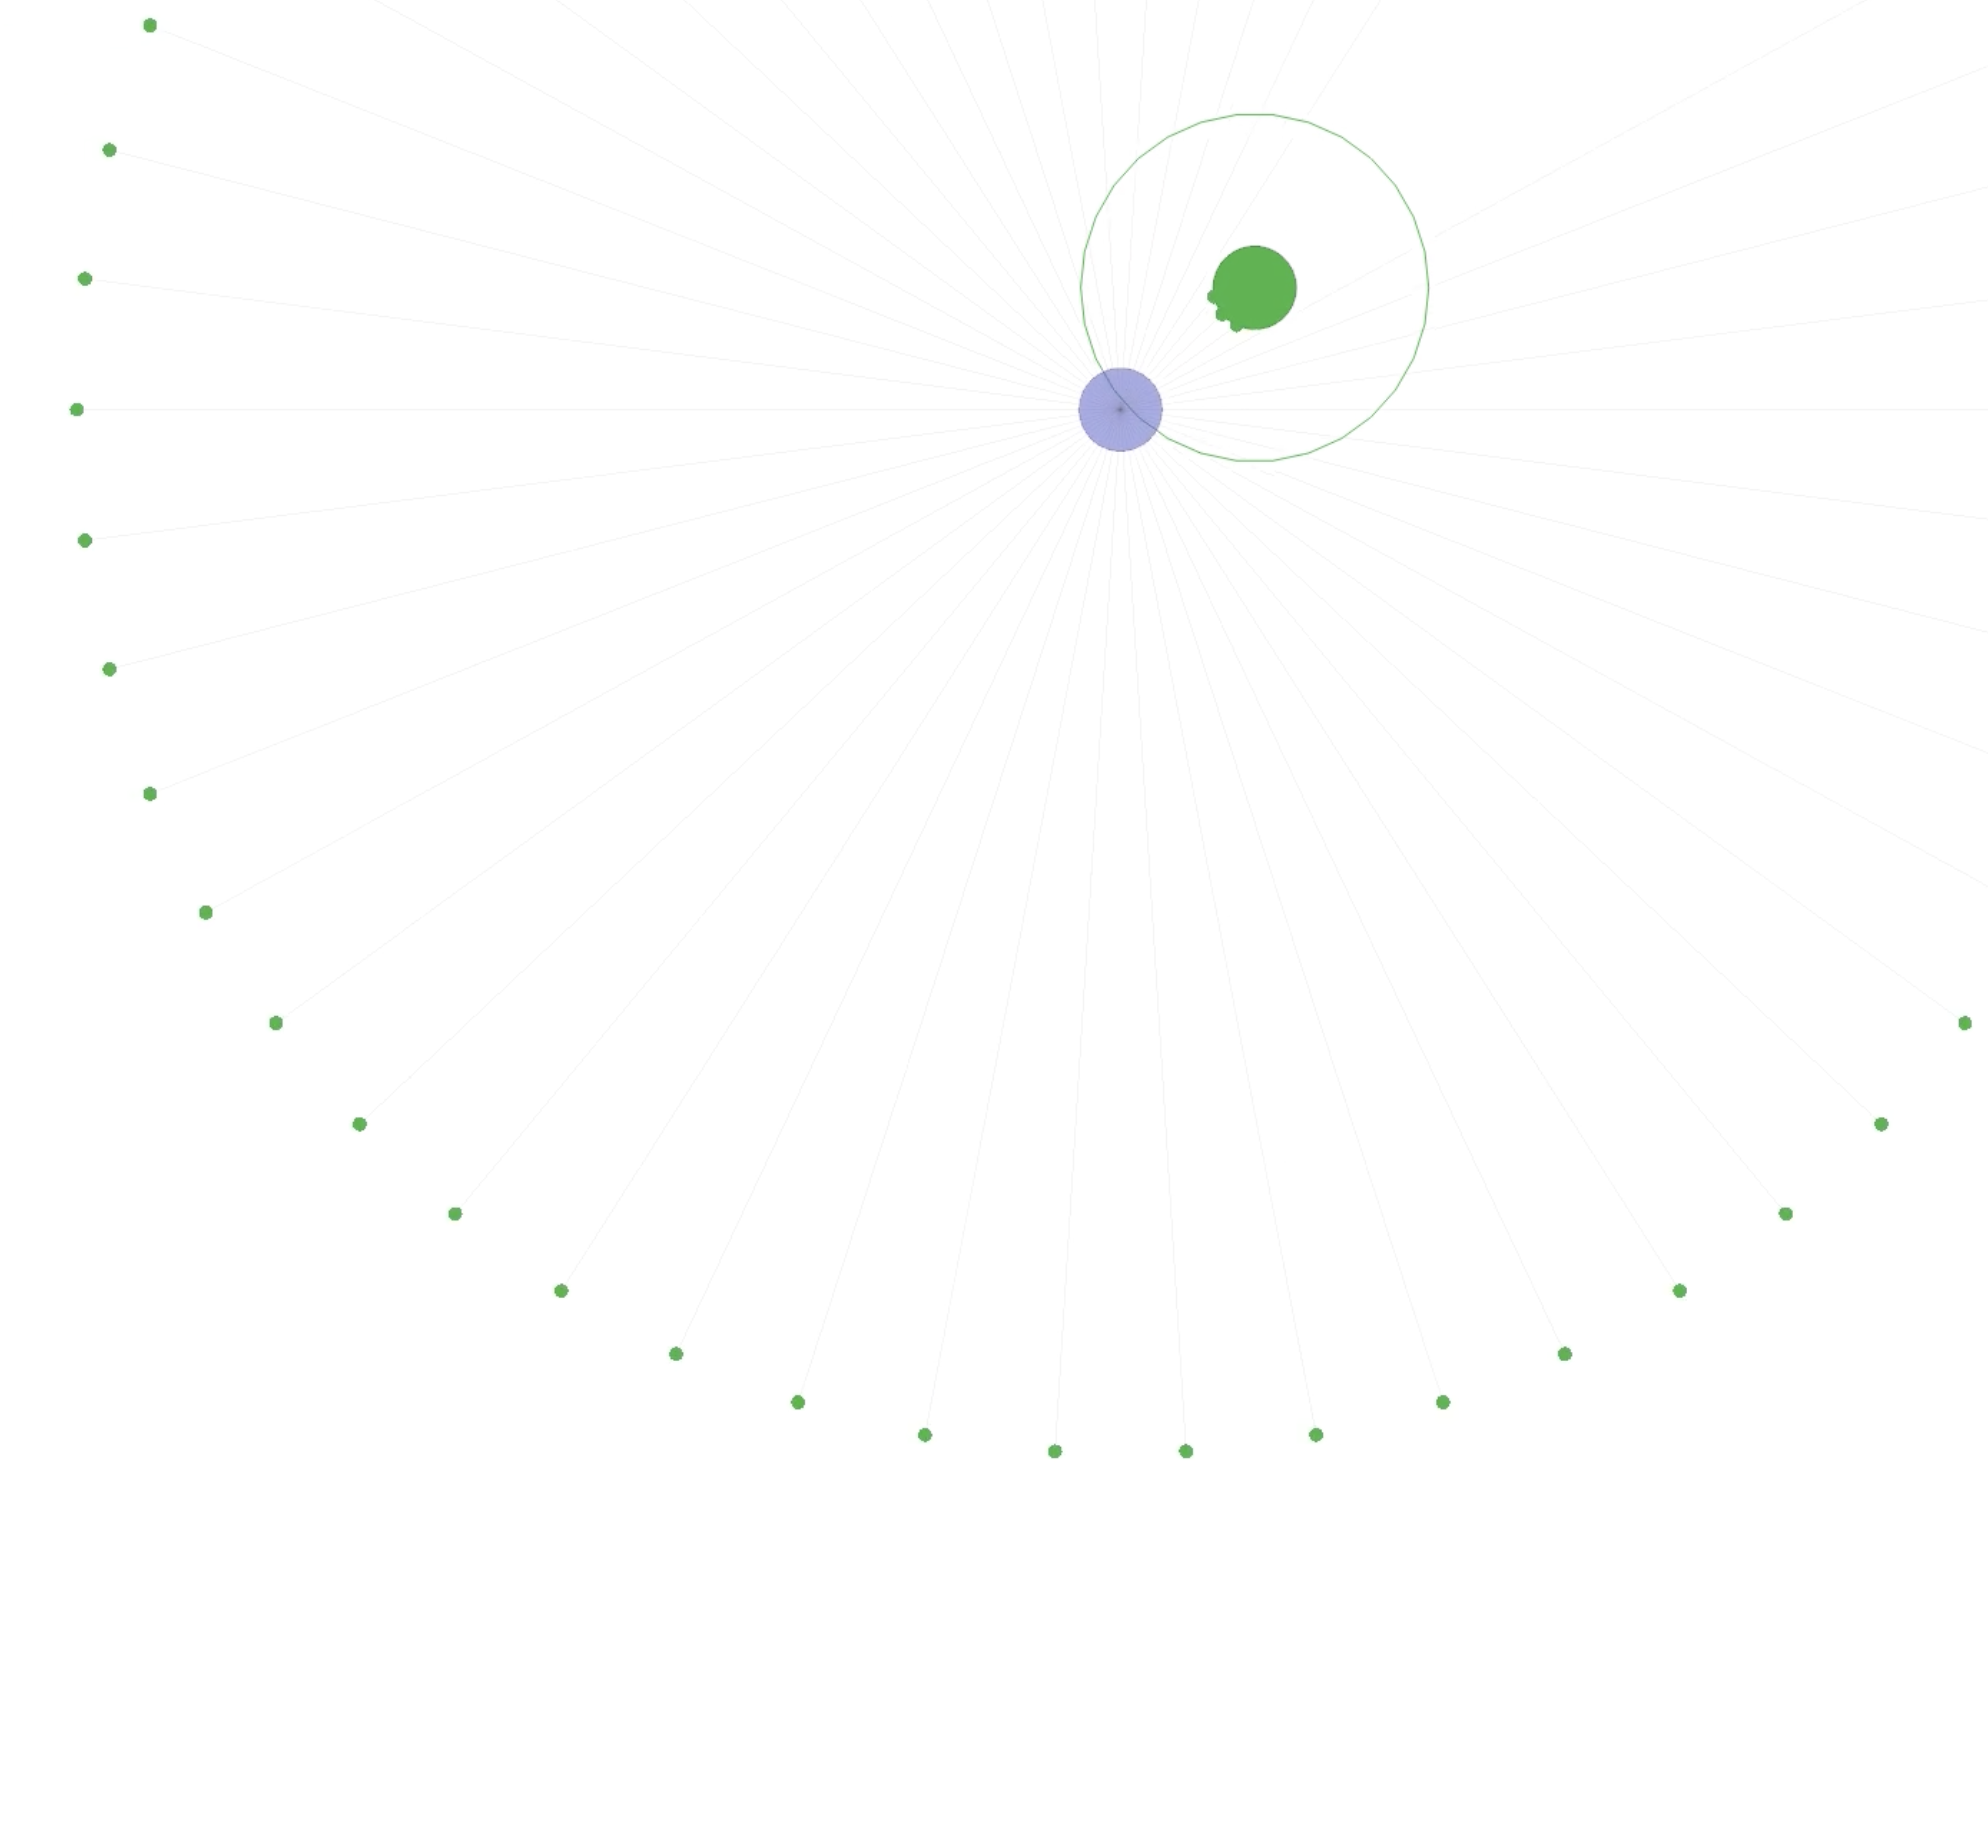
\includegraphics[width=\textwidth]{img/1_agent_3.png}
			\caption{End of simulation} 
		\end{subfigure}
		\caption{Different stages of a simulation with one agent and 8 targets}
		\label{fig:m}
	\end{figure}

	\begin{block}{Evaluation with one agent}
		To assess the agents' performance in practical scenarios, I conducted evaluations with varying numbers of agents and targets. In a scenario involving one agent and eight targets [\ref{fig:m}], the results indicated the following:
			\begin{itemize}
			\item On average, it took approximately 10 steps for the agent to remove the first target, reflecting a quick initiation of the cleaning process [\ref{fig:d}].
			\item Removal of half the targets occurred, on average, in approximately 170 steps, demonstrating consistent progress [\ref{fig:e}].
			\item To remove all eight targets, agents required an average of around 1440 steps, highlighting the complexity of clearing the entire environment [\ref{fig:f}].
			\end{itemize}
	\end{block}

	\begin{figure}
		\centering
		\begin{subfigure}[b]{0.45\textwidth}
			\centering
			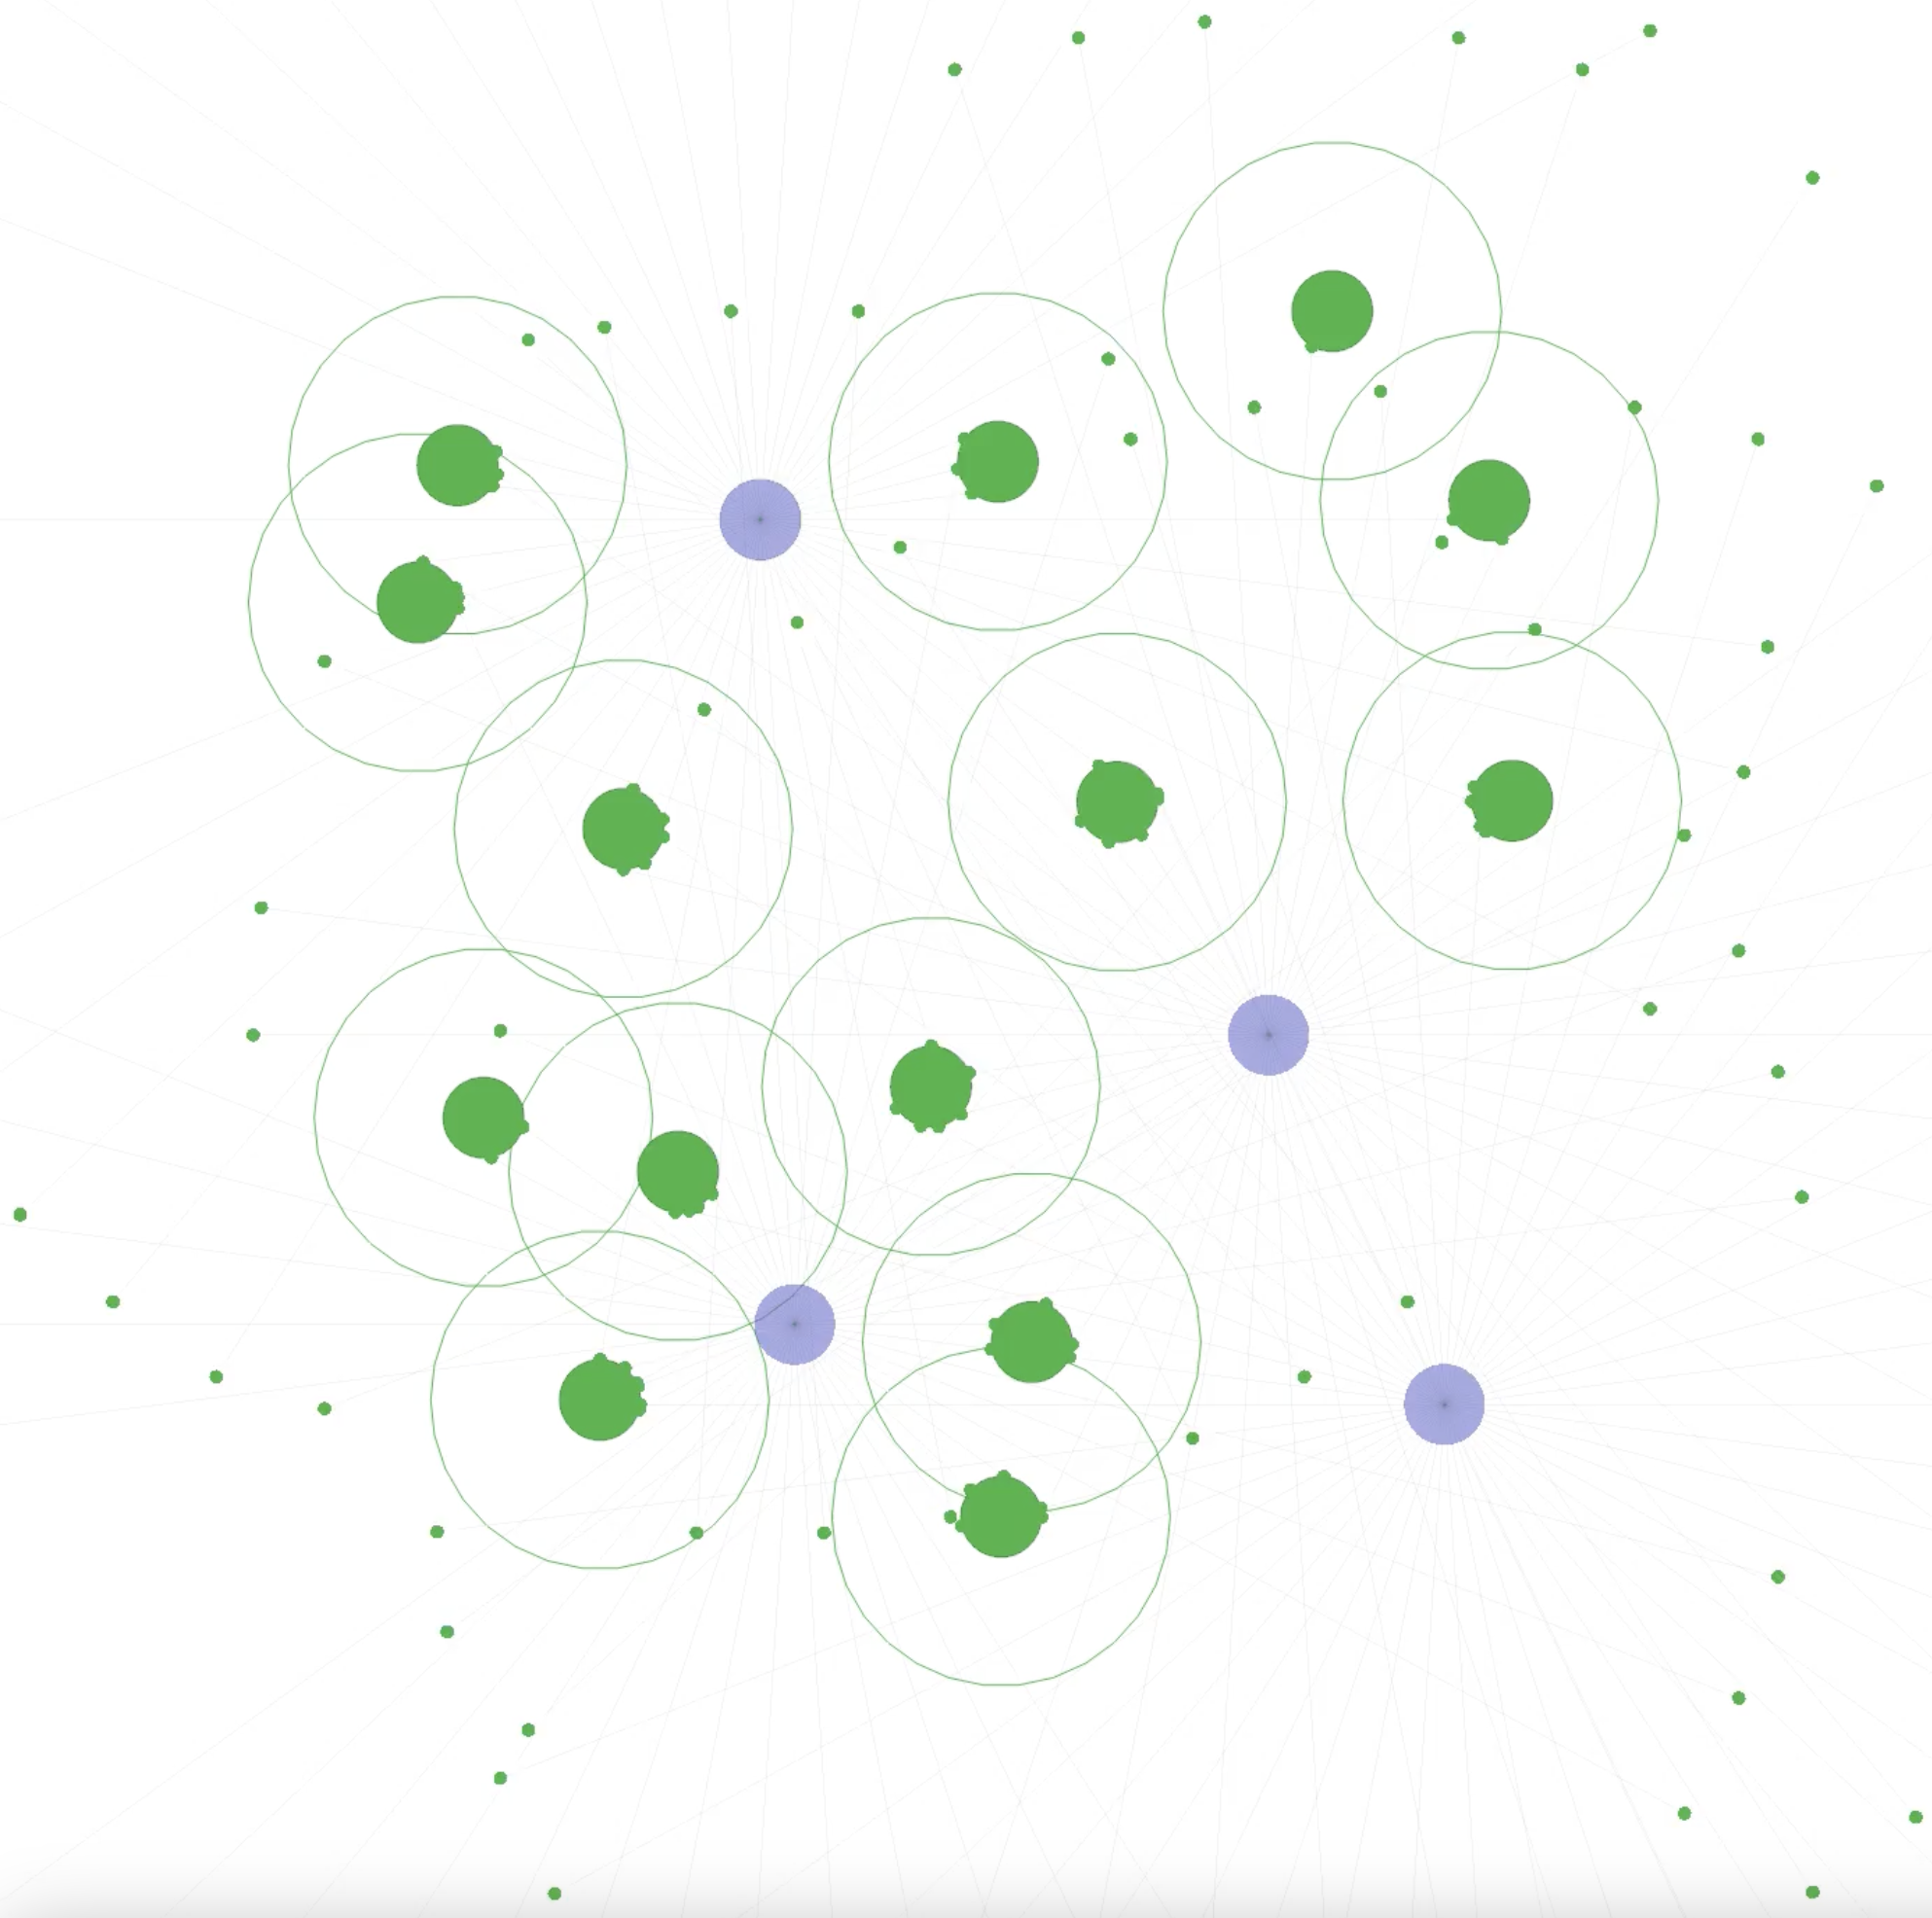
\includegraphics[width=\textwidth]{img/4_agents_1.png}
			\caption{Beginning of simulation}
		\end{subfigure}
		\hfill
		\begin{subfigure}[b]{0.45\textwidth}
			\centering
			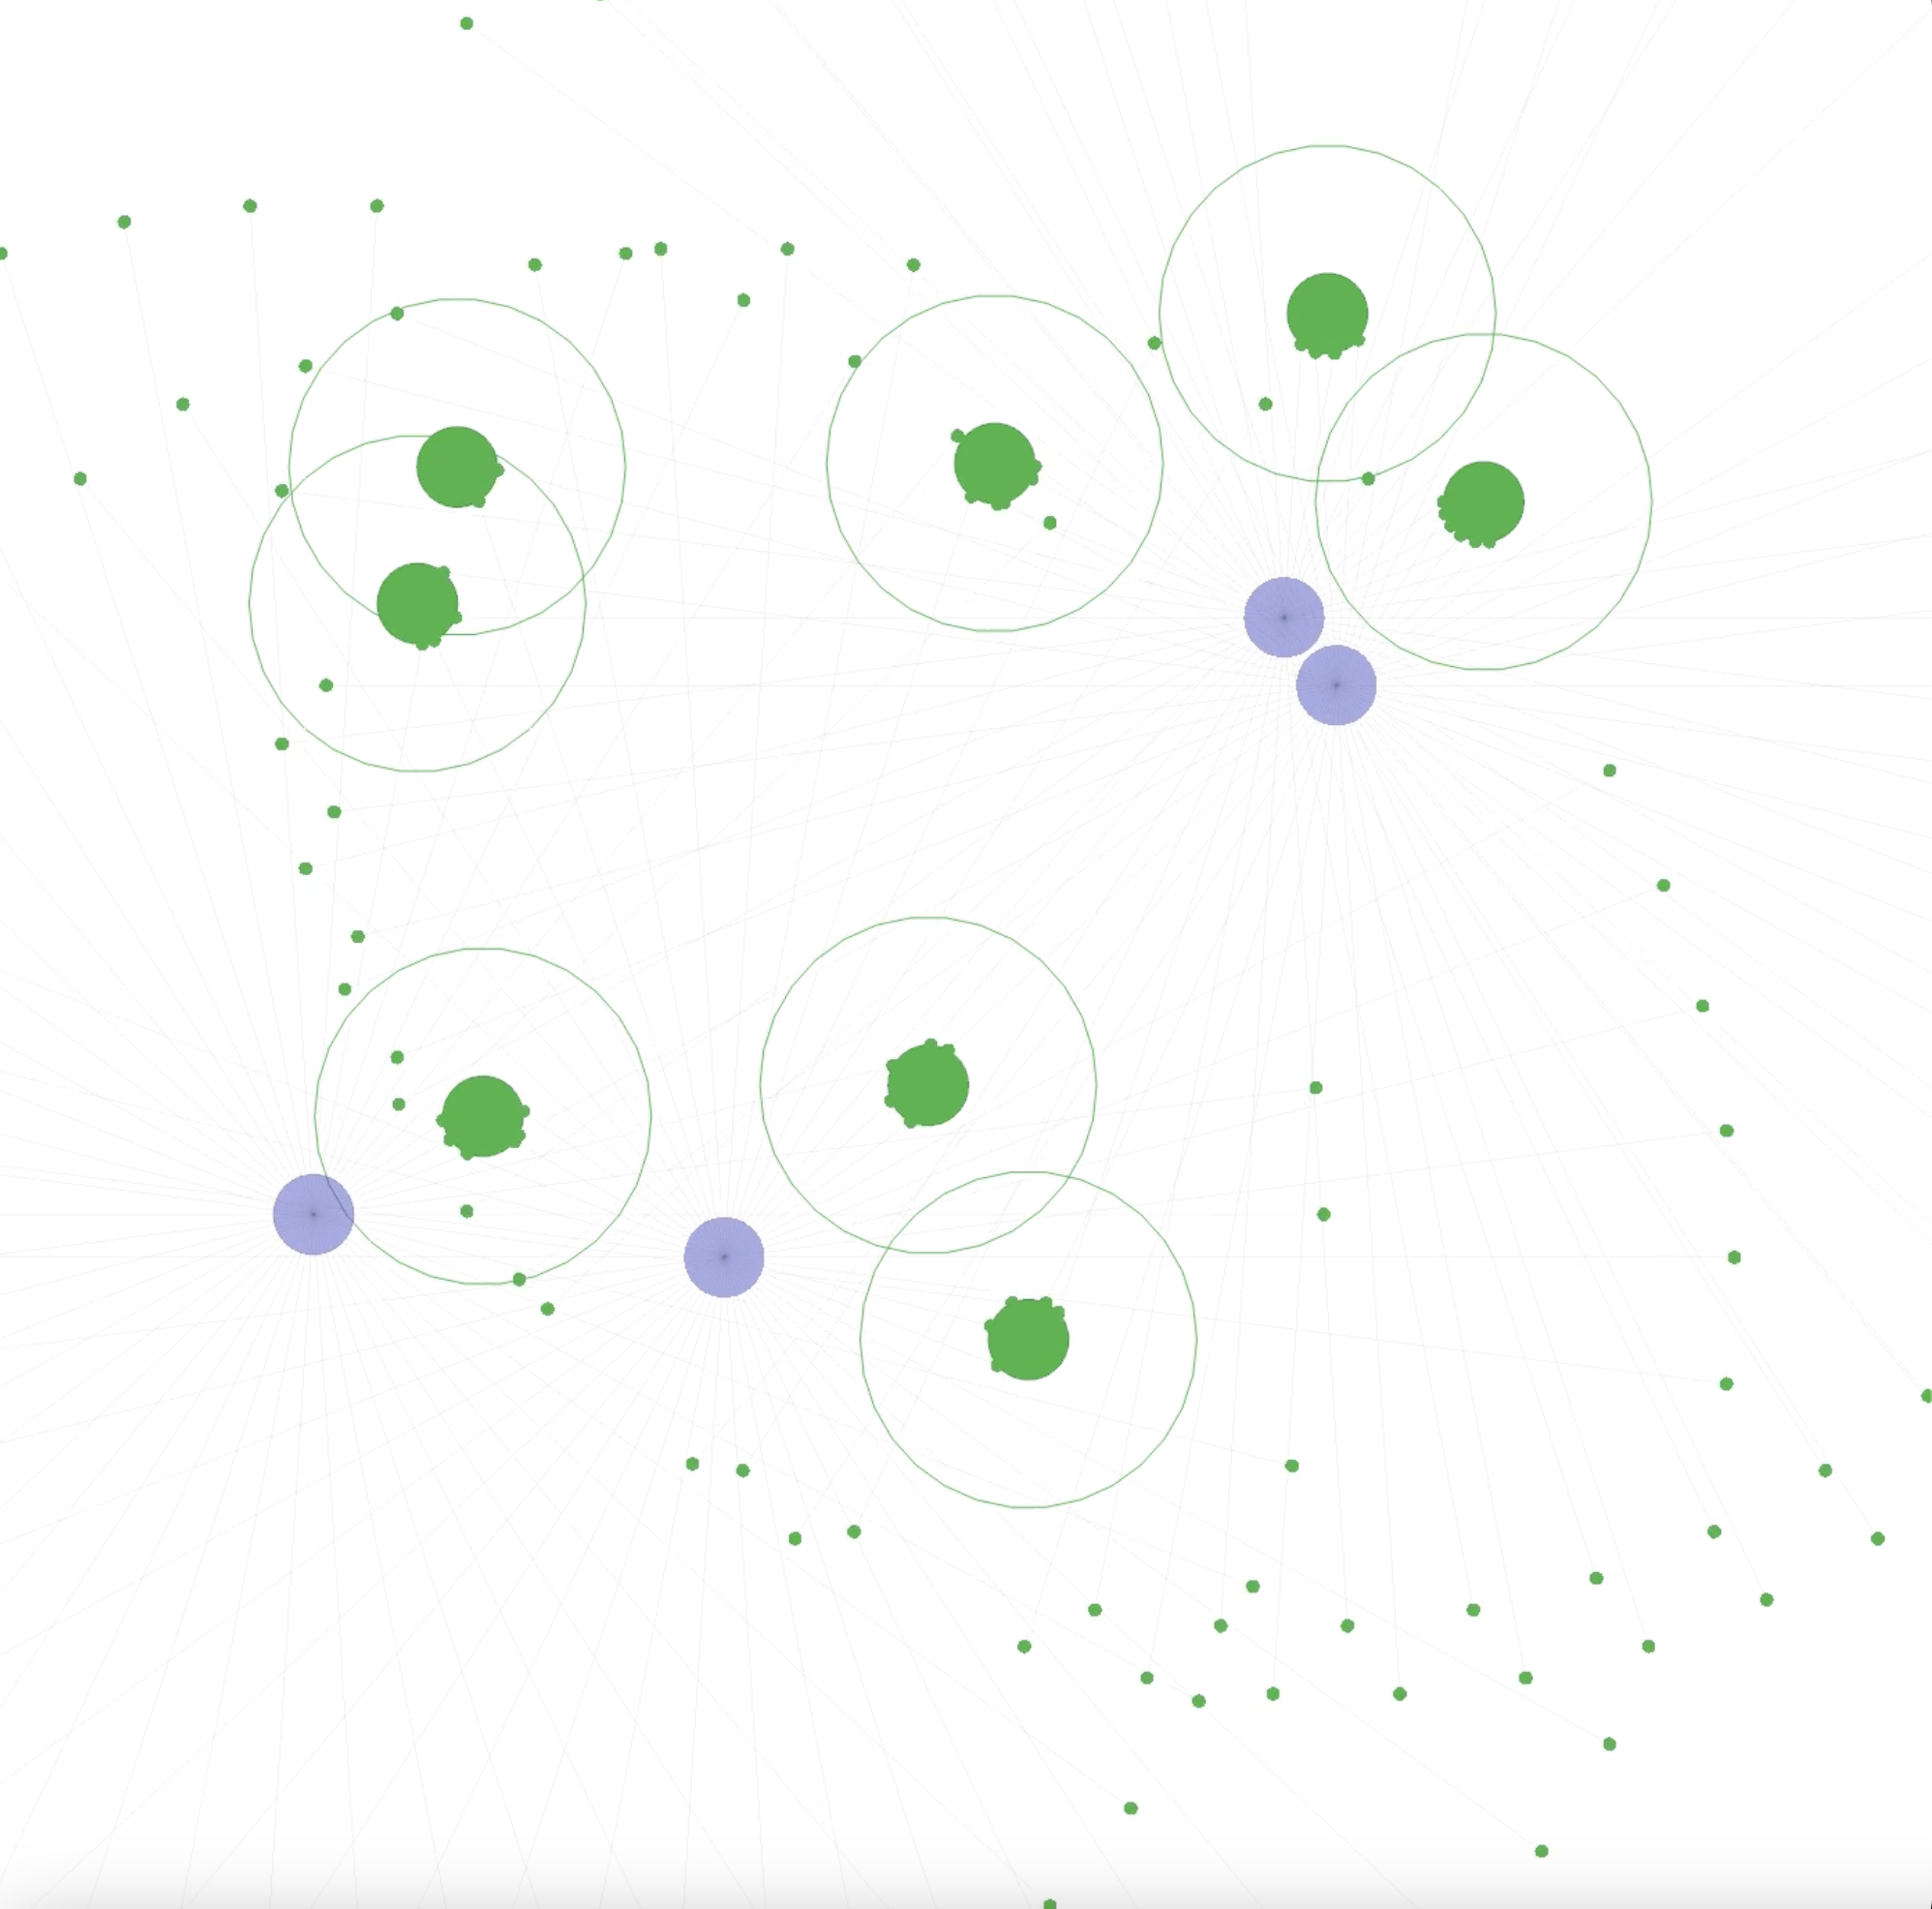
\includegraphics[width=\textwidth]{img/4_agents_2.png}
			\caption{Half simulation}
		\end{subfigure}
		\hfill
		\begin{subfigure}[b]{0.45\textwidth}
			\centering
			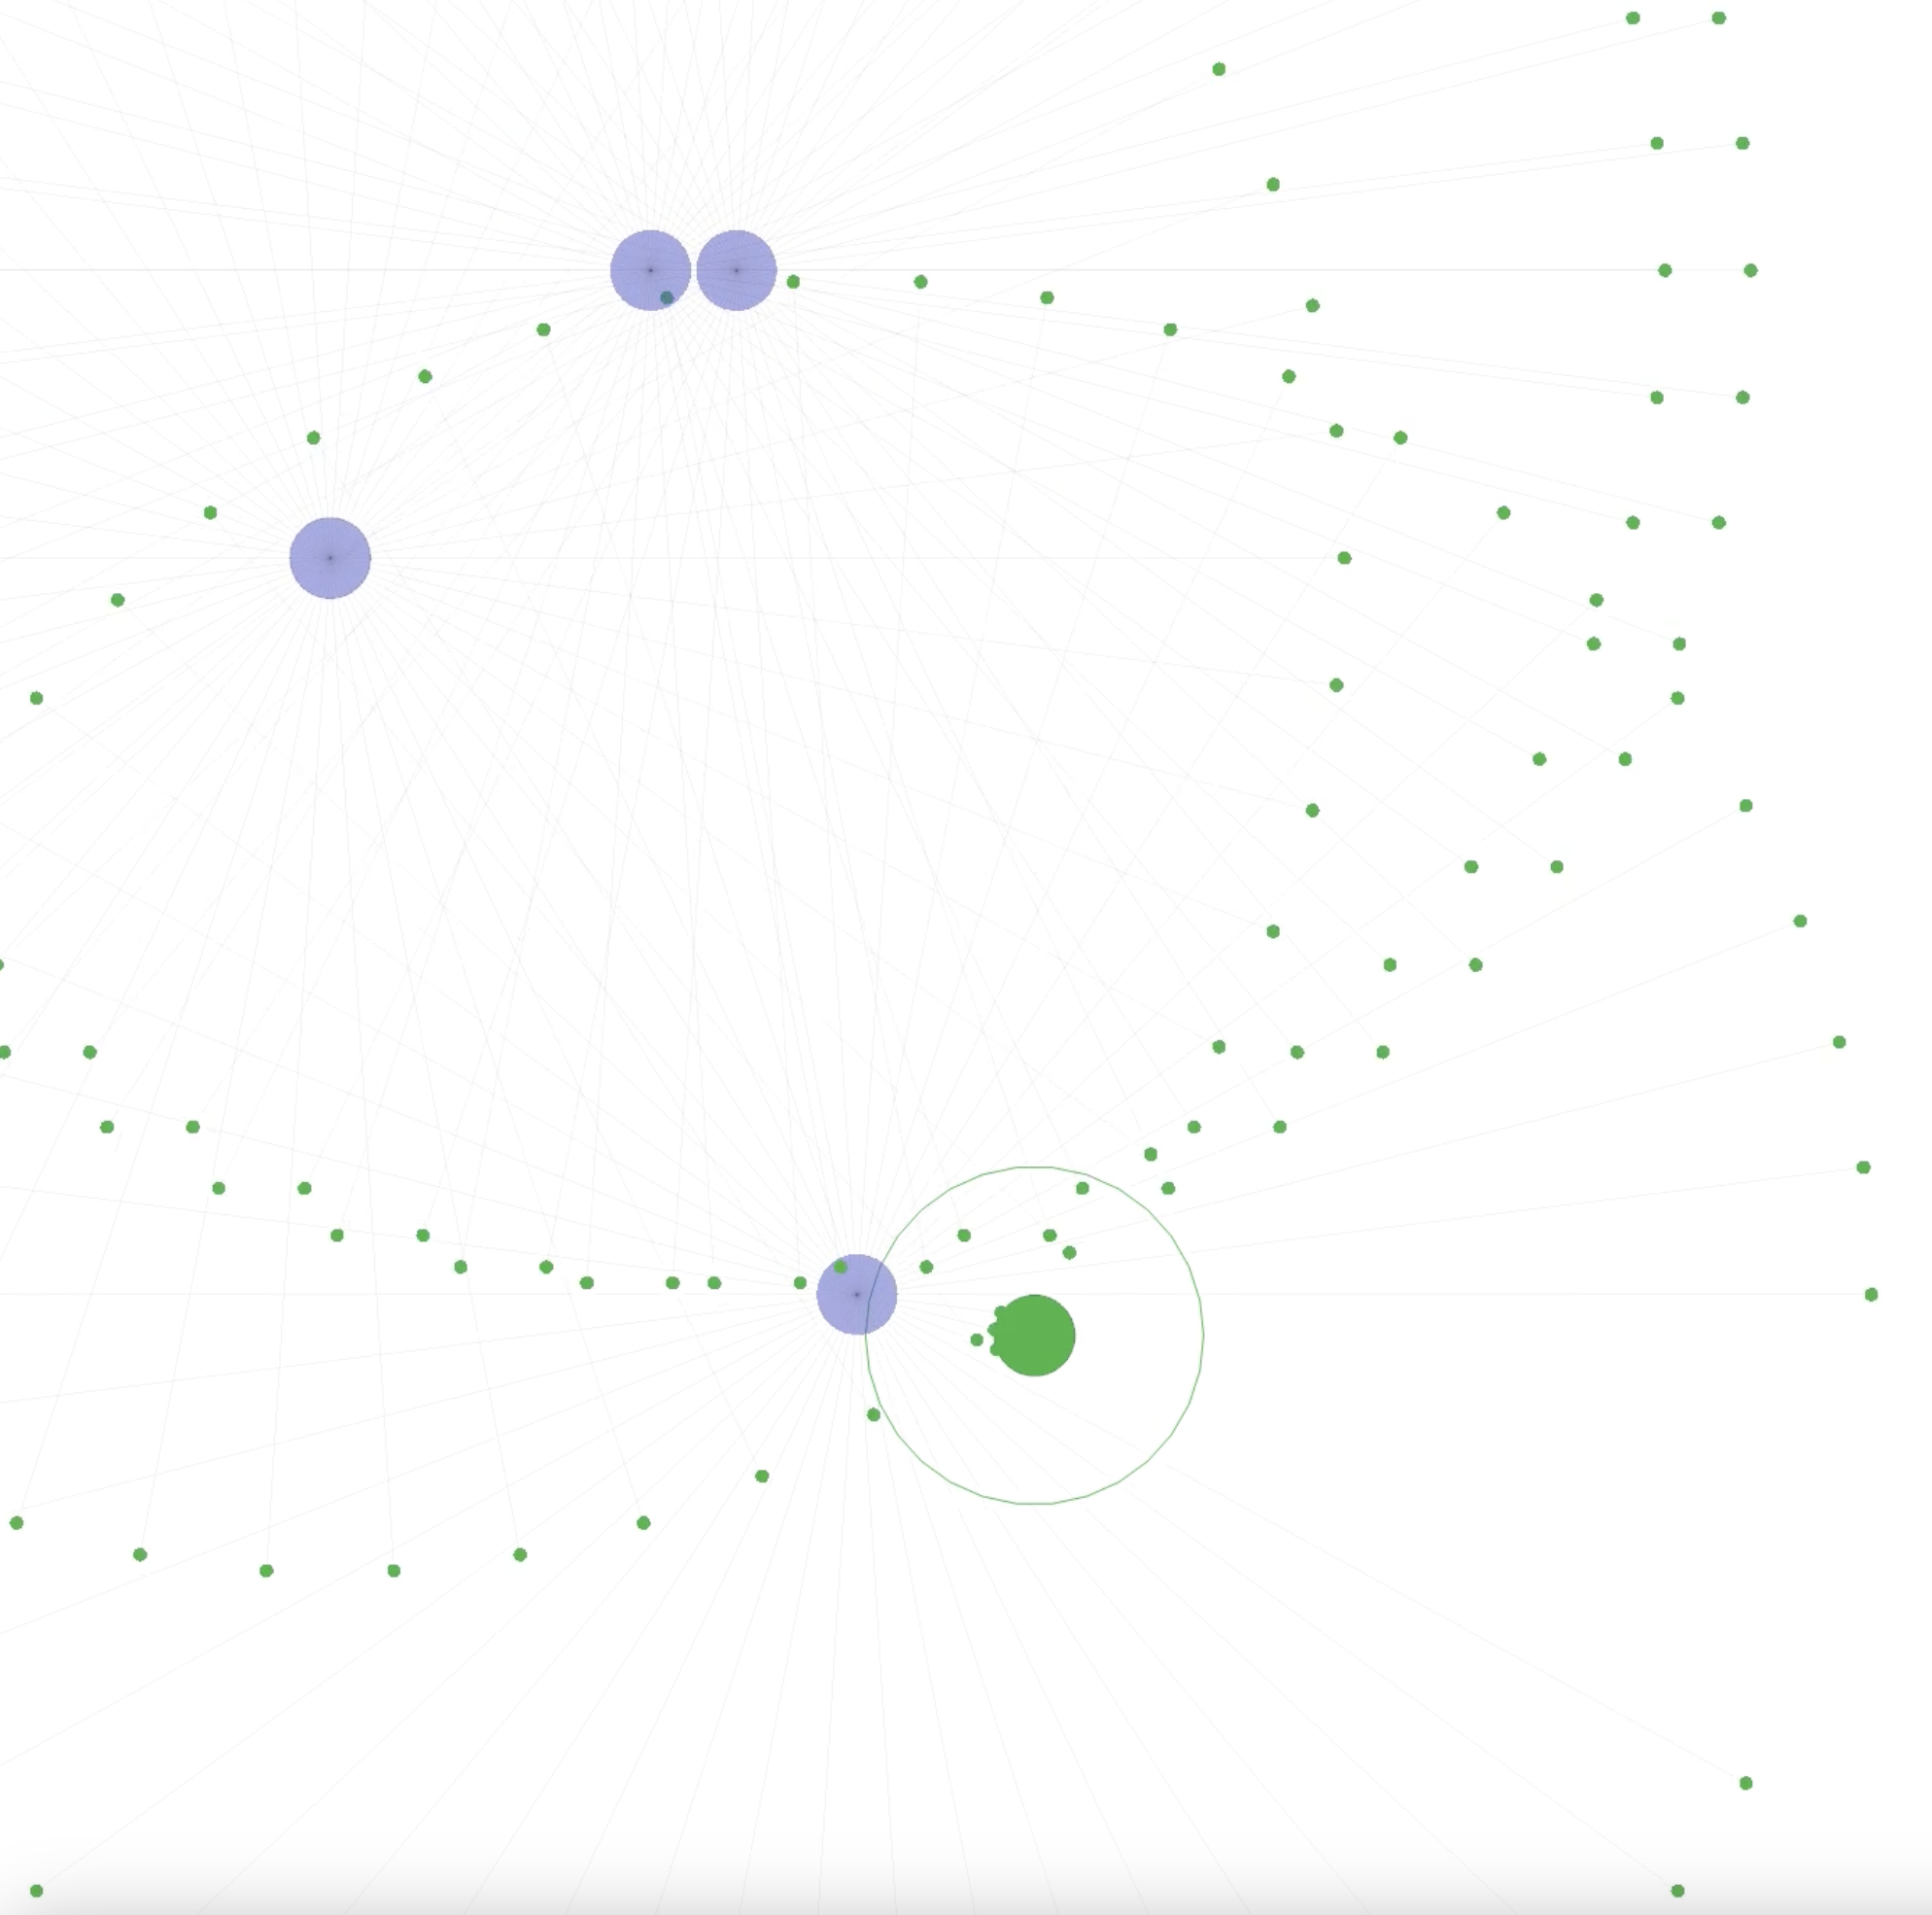
\includegraphics[width=\textwidth]{img/4_agents_3.png}
			\caption{End of simulation} 
		\end{subfigure}
		\caption{Different stages of a simulation with four agent and 14 targets}
		\label{fig:n}
	  \end{figure}

	\begin{block}{Evaluation with many agents}
		In a more challenging scenario with four agents and fourteen targets [\ref{fig:n}], the outcomes were as follows:
\begin{itemize}
  \item Agents demonstrated improved collaboration, taking an average of about 400 steps to clear all fourteen targets.
  \item The first target was removed in an average of 10 steps, emphasizing swift task initiation.
  \item Removal of half the targets was achieved in approximately 240 steps, showcasing efficient teamwork among agents.
\end{itemize}
	\end{block}

	\begin{figure}
		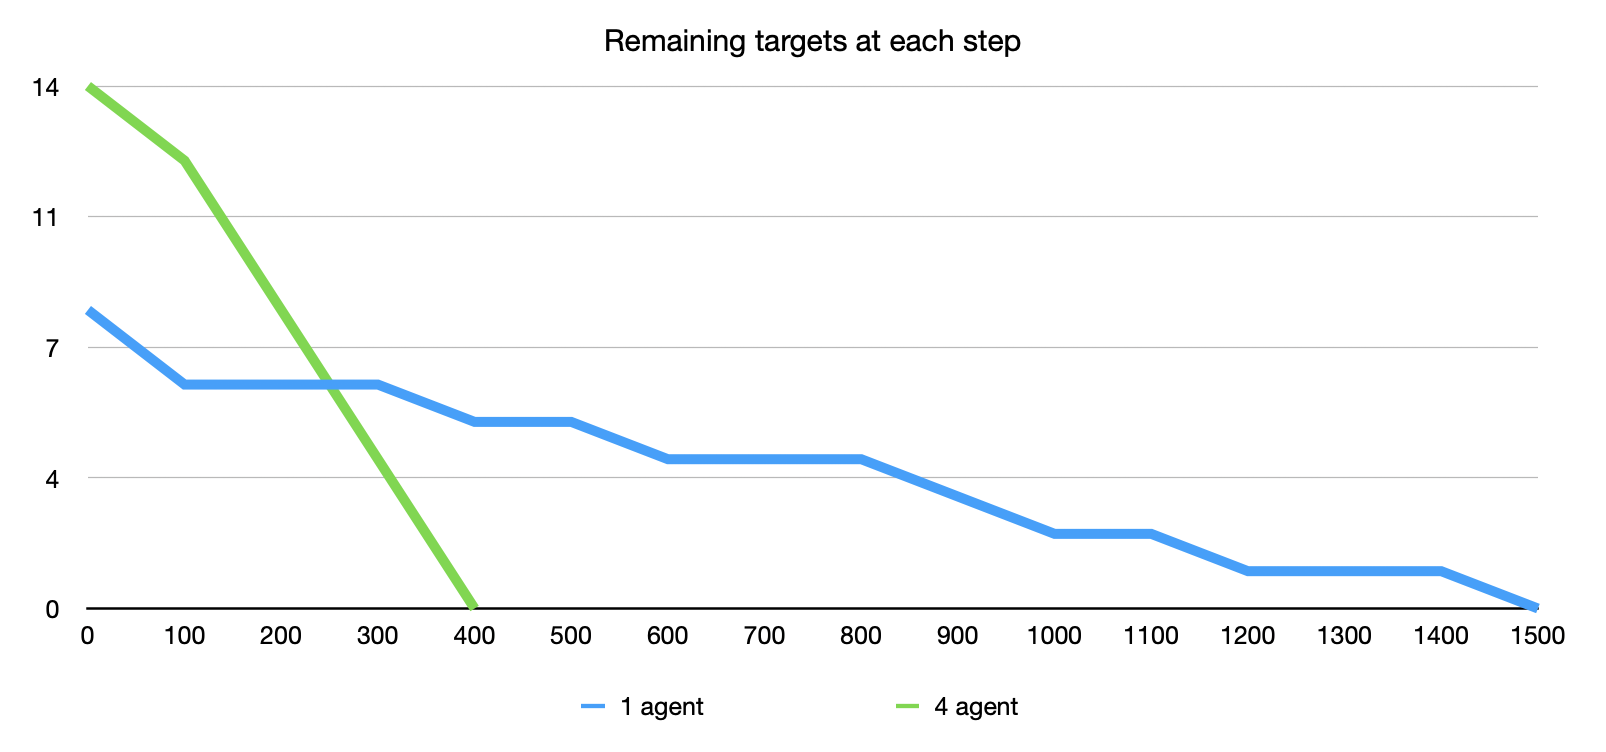
\includegraphics[width=\textwidth]{img/active-targets-per-step.png}
		\caption{Remaining targets at each step}
		\label{fig:o}
		\end{figure}
\end{frame}
%/////////


%===============================================================================
\section*{}
%===============================================================================

%/////////
\frame{\titlepage}
%/////////

%===============================================================================
\section*{\refname}
%===============================================================================

%%%%
\setbeamertemplate{page number in head/foot}{}
%/////////
\begin{frame}[c,noframenumbering, allowframebreaks]{\refname}
%\begin{frame}[t,allowframebreaks,noframenumbering]{\refname}
	\tiny
	\nocite{*}
	\printbibliography
\end{frame}
%/////////

%%%%%%%%%%%%%%%%%%%%%%%%%%%%%%%%%%%%%%%%%%%%%%%%%%%%%%%%%%%%%%%%%%%%%%%%%%%%%%%%
\end{document}
%%%%%%%%%%%%%%%%%%%%%%%%%%%%%%%%%%%%%%%%%%%%%%%%%%%%%%%%%%%%%%%%%%%%%%%%%%%%%%%%
